% =====================================================================================
%  MAT 451E - Assignment 2: Character-Level GPT (training and generation)
%  Report of Ömer Kahyaoğlu (090240741, kahyaoglu20@itu.edu.tr)
%  Build:  python report/build_assets.py   (regenerates every measured number)
%          cd report && pdflatex report && pdflatex report && pdflatex report
% =====================================================================================
\documentclass[11pt,a4paper]{article}
\usepackage[T1]{fontenc}
\usepackage[utf8]{inputenc}
\usepackage{lmodern}
\usepackage[a4paper,margin=2.1cm,headheight=14pt]{geometry}
\usepackage{amsmath,amssymb,mathtools,bm}
\usepackage{booktabs,longtable,array,tabularx,multirow}
\usepackage{graphicx}
\usepackage[dvipsnames]{xcolor}
\usepackage{listings}
\usepackage{fvextra}
\usepackage{seqsplit}
\usepackage{tikz}
\usetikzlibrary{arrows.meta,positioning,calc,fit}
\usepackage[most]{tcolorbox}
\usepackage{caption}
\usepackage{enumitem}
\usepackage{fancyhdr}
\usepackage{microtype}
\usepackage[hidelinks,
  pdftitle={MAT 451E Assignment 2 -- Character-Level GPT: Training and Generation},
  pdfauthor={Ömer Kahyaoğlu (090240741)},
  pdfsubject={Mathematical Foundations of Large Language Models, Istanbul Technical University},
  pdfkeywords={character-level GPT, residual Transformer block, GELU, cross-entropy, Adam, autoregressive sampling},
  pdfcreator={LaTeX with hyperref}]{hyperref}
\widowpenalty=10000 \clubpenalty=10000 \predisplaypenalty=1000

\graphicspath{{../results/python/figures/}{../results/matlab/figures/}}
\newcommand{\Ncorpus}{1\,115\,394}
\newcommand{\Vsize}{65}
\newcommand{\Ntr}{1\,003\,854}
\newcommand{\Nva}{111\,540}
\newcommand{\Shasum}{86c4e6aa9db7c042\dots}
\newcommand{\ShasumFull}{86c4e6aa9db7c042ec79f339dcb96d42b0075e16b8fc2e86bf0ca57e2dc565ed}
\newcommand{\Ptotal}{112\,000}
\newcommand{\logV}{4.174387}
\newcommand{\GeluApproxM}{-0.158808009}
\newcommand{\GeluExactM}{-0.158655254}
\newcommand{\GeluApproxP}{+0.841191991}
\newcommand{\GeluExactP}{+0.841344746}
\newcommand{\GeluDiff}{\ensuremath{1.53\times10^{-4}}}
\newcommand{\GeluGridMax}{\ensuremath{4.7\times10^{-4}}}
\newcommand{\GeluGradAuto}{\ensuremath{2.2\times10^{-16}}}
\newcommand{\GeluGradFD}{\ensuremath{9.5\times10^{-11}}}
\newcommand{\ResJacErr}{\ensuremath{1.7\times10^{-10}}}
\newcommand{\FFNTermsErr}{\ensuremath{6.7\times10^{-16}}}
\newcommand{\BtwoRel}{\ensuremath{1.4\times10^{-13}}}
\newcommand{\BtwoStrict}{\ensuremath{1.4\times10^{-9}}}
\newcommand{\CEexLSEa}{2.169846}
\newcommand{\CEexLSEb}{1.551445}
\newcommand{\CEexNLLa}{0.169846}
\newcommand{\CEexNLLb}{0.551445}
\newcommand{\CEexL}{0.360645366744}
\newcommand{\CEexRef}{0.360645366744}
\newcommand{\ShiftStable}{0.360645366744}
\newcommand{\ShiftNaive}{nan}
\newcommand{\OrdPy}{(1, 2, 3, 4, 5, 6)}
\newcommand{\OrdMl}{(1, 4, 2, 5, 3, 6)}
\newcommand{\LOrdPy}{1.950721077065}
\newcommand{\LOrdMl}{1.950721077065}
\newcommand{\LOrdMix}{2.907759547899}
\newcommand{\LOrdPerm}{1.950721077065}
\newcommand{\BoneL}{0.767528364331}
\newcommand{\BoneRef}{0.767528364331}
\newcommand{\AdamMone}{0.02}
\newcommand{\AdamVone}{4.00\times10^{-5}}
\newcommand{\AdamMhat}{0.2}
\newcommand{\AdamVhat}{0.04}
\newcommand{\AdamUpd}{-0.000999999950}
\newcommand{\FullLoss}{4.196727}
\newcommand{\FullErr}{\ensuremath{1.4\times10^{-16}}}
\newcommand{\WErowsHit}{57}
\newcommand{\Sepoch}{490}
\newcommand{\StotalFull}{24\,500}
\newcommand{\FDbestDelta}{1\times10^{-5}}
\newcommand{\FDatFive}{\ensuremath{8.1\times10^{-11}}}
\newcommand{\FDbest}{\ensuremath{8.1\times10^{-11}}}
\newcommand{\SynFirst}{0.6417}
\newcommand{\SynLast}{\ensuremath{1.8\times10^{-3}}}
\newcommand{\SynSteps}{300}
\newcommand{\SynVal}{\ensuremath{1.8\times10^{-3}}}
\newcommand{\Stotal}{24\,500}
\newcommand{\TrainMinutes}{61.5}
\newcommand{\Lvalfixed}{1.6339}
\newcommand{\Ltrainfixed}{1.3880}
\newcommand{\Lgap}{+0.2459}
\newcommand{\Lvalinit}{4.1972}
\newcommand{\NfixedVa}{512}
\newcommand{\NfixedTr}{512}
\newcommand{\FirstTrain}{4.1967}
\newcommand{\FirstVal}{4.0313}
\newcommand{\LastTrain}{1.4138}
\newcommand{\LastVal}{1.7188}
\newcommand{\NumEvals}{491}
\newcommand{\Perplexity}{5.12}
\newcommand{\PerplexityInit}{66.50}
\newcommand{\BitsPerChar}{2.357}
\newcommand{\NumPreviews}{10}
\newcommand{\EpochsRun}{50}
\newcommand{\ValNoise}{0.135}
\newcommand{\ProbOne}{(0.665241, 0.244728, 0.090031)}
\newcommand{\EntOne}{0.8324}
\newcommand{\ProbHalf}{(0.866813, 0.117310, 0.015876)}
\newcommand{\EntHalf}{0.4411}
\newcommand{\ProbTwo}{(0.506480, 0.307196, 0.186324)}
\newcommand{\EntTwo}{1.0202}
\newcommand{\SamplerFreq}{(0.6635, 0.2456, 0.0910)}
\newcommand{\LzeroInit}{4.196727}
\newcommand{\BfiveErr}{\ensuremath{0}}
\newcommand{\PyVersion}{3.13.17}
\newcommand{\NumpyVersion}{2.5.3}
\newcommand{\MplVersion}{3.11.2}
\newcommand{\Platform}{Linux-6.18.44-fc-v153-x86\_64-with-glibc2.39}
\newcommand{\PySeconds}{61.9}
\newcommand{\PyPassed}{67}
\newcommand{\NChecks}{67}
\newcommand{\MlRun}{1}
\newcommand{\MlPassed}{67}
\newcommand{\MlVersion}{24.1.0.2537033 (R2024a)}
\newcommand{\MlGrad}{dlgradient}
\newcommand{\MlToolbox}{24.1}
\newcommand{\MlComputer}{PCWIN64}
\newcommand{\MlLvalfixed}{1.6375}
\newcommand{\MlLtrainfixed}{1.3906}
\newcommand{\MlLvalinit}{4.1945}
\newcommand{\MlLgap}{+0.2469}
\newcommand{\MlPerplexity}{5.14}
\newcommand{\MlBitsPerChar}{2.362}
\newcommand{\MlStotal}{24\,500}
\newcommand{\MlMinutes}{51.7}
\newcommand{\MlTotalMinutes}{51.9}
\newcommand{\MlValDiff}{0.0036}

\newcommand{\SmallWone}{\begin{bmatrix}0.4 & -0.3 & 0.2 & 0.1 & -0.5 & 0.6 & 0.0 & 0.3 \\ 0.1 & 0.2 & -0.4 & 0.5 & 0.3 & -0.1 & 0.7 & -0.2\end{bmatrix}}
\newcommand{\SmallWtwo}{\begin{bmatrix}0.30 & -0.20 \\ 0.10 & 0.40 \\ -0.50 & 0.20 \\ 0.20 & 0.10 \\ 0.00 & -0.30 \\ 0.40 & 0.00 \\ -0.10 & 0.50 \\ 0.20 & 0.20\end{bmatrix}}
\newcommand{\SmallJ}{\begin{bmatrix}0.100 & -0.250 & 0.400 & -0.250 & -0.550 & 0.200 & -0.600 & 0.350\end{bmatrix}}
\newcommand{\SmallgJ}{\begin{bmatrix}0.0540 & -0.1003 & 0.2622 & -0.1003 & -0.1602 & 0.1159 & -0.1646 & 0.2229\end{bmatrix}}
\newcommand{\SmallG}{\begin{bmatrix}0.01239 & -0.04819\end{bmatrix}}
\newcommand{\SmallBone}{\begin{bmatrix}0.0 & 0.1 & -0.1 & 0.2 & 0.0 & -0.2 & 0.1 & 0.0\end{bmatrix}}
\newcommand{\SmallBtwo}{\begin{bmatrix}0.05 & -0.05\end{bmatrix}}
\newcommand{\BlockF}{\begin{bmatrix}2.90 & 0.00 & 0.00 & 0.00 \\ 2.53 & 0.06 & 0.00 & 0.00 \\ 1.32 & 0.05 & 0.04 & 0.00 \\ 0.31 & 0.07 & 0.03 & 0.05\end{bmatrix}}
\newcommand{\BlockG}{\begin{bmatrix}0.15 & 0.00 & 0.00 & 0.00 \\ 0.00 & 0.26 & 0.00 & 0.00 \\ 0.00 & 0.00 & 0.28 & 0.00 \\ 0.00 & 0.00 & 0.00 & 0.22\end{bmatrix}}
\newcommand{\CEexGrad}{\begin{bmatrix}-0.078103 & 0.057098 & 0.021005 \\ 0.105971 & -0.211942 & 0.105971\end{bmatrix}}
\newcommand{\BoneP}{\begin{bmatrix}0.333333 & 0.333333 & 0.333333 \\ 0.500000 & 0.250000 & 0.250000 \\ 0.200000 & 0.600000 & 0.200000\end{bmatrix}}
\newcommand{\BoneGrad}{\begin{bmatrix}-0.222222 & 0.111111 & 0.111111 \\ -0.166667 & 0.083333 & 0.083333 \\ 0.066667 & -0.133333 & 0.066667\end{bmatrix}}
\newcommand{\BenchP}{\begin{bmatrix}0.333333333 & 0.333333333 & 0.333333333 \\ 0.333333333 & 0.333333333 & 0.333333333\end{bmatrix}}
\newcommand{\BenchGZ}{\begin{bmatrix}\tfrac{1}{6} & -\tfrac{1}{3} & \tfrac{1}{6} \\ \tfrac{1}{6} & \tfrac{1}{6} & -\tfrac{1}{3}\end{bmatrix}}
\newcommand{\BenchGW}{\begin{bmatrix}\tfrac{1}{6} & -\tfrac{1}{3} & \tfrac{1}{6} \\ \tfrac{1}{6} & \tfrac{1}{6} & -\tfrac{1}{3}\end{bmatrix}}
\newcommand{\BenchWnew}{\begin{bmatrix}-0.001000000 & +0.001000000 & -0.001000000 \\ -0.001000000 & -0.001000000 & +0.001000000\end{bmatrix}}
\newcommand{\BenchL}{1.098612288668}
\newcommand{\BthreeThetaZero}{\begin{bmatrix}0.547402 & -0.970805 & 0.202290 \\ 0.250126 & -0.517967 & -0.561857\end{bmatrix}}
\newcommand{\BthreeG}{\begin{bmatrix}0.50 & -0.20 & 0.01 \\ -1.50 & 0.30 & 2.00\end{bmatrix}}
\newcommand{\BthreeM}{\begin{bmatrix}0.0500 & -0.0200 & 0.0010 \\ -0.1500 & 0.0300 & 0.2000\end{bmatrix}}
\newcommand{\BthreeV}{\begin{bmatrix}0.0002500 & 0.0000400 & 0.0000001 \\ 0.0022500 & 0.0000900 & 0.0040000\end{bmatrix}}
\newcommand{\BthreeThetaOne}{\begin{bmatrix}0.546402 & -0.969805 & 0.201290 \\ 0.251126 & -0.518967 & -0.562857\end{bmatrix}}
\newcommand{\BthreeErr}{\ensuremath{1.3\times10^{-23}}}

% measured value of every verification check (generated)
\expandafter\def\csname chkpy@D.1\endcsname{\ensuremath{0}}
\expandafter\def\csname chkml@D.1\endcsname{\ensuremath{0}}
\expandafter\def\csname chkpy@D.2\endcsname{\ensuremath{0}}
\expandafter\def\csname chkml@D.2\endcsname{\ensuremath{0}}
\expandafter\def\csname chkpy@D.3\endcsname{\ensuremath{0}}
\expandafter\def\csname chkml@D.3\endcsname{\ensuremath{0}}
\expandafter\def\csname chkpy@D.4\endcsname{\ensuremath{0}}
\expandafter\def\csname chkml@D.4\endcsname{\ensuremath{0}}
\expandafter\def\csname chkpy@Q1.1\endcsname{\ensuremath{2.8\times10^{-17}}}
\expandafter\def\csname chkml@Q1.1\endcsname{\ensuremath{2.8\times10^{-17}}}
\expandafter\def\csname chkpy@Q1.2\endcsname{\ensuremath{1.5\times10^{-4}}}
\expandafter\def\csname chkml@Q1.2\endcsname{\ensuremath{1.5\times10^{-4}}}
\expandafter\def\csname chkpy@Q1.3\endcsname{\ensuremath{2.2\times10^{-16}}}
\expandafter\def\csname chkml@Q1.3\endcsname{\ensuremath{2.2\times10^{-16}}}
\expandafter\def\csname chkpy@Q1.4\endcsname{\ensuremath{1.7\times10^{-10}}}
\expandafter\def\csname chkml@Q1.4\endcsname{\ensuremath{2.2\times10^{-10}}}
\expandafter\def\csname chkpy@Q1.5\endcsname{\ensuremath{0}}
\expandafter\def\csname chkml@Q1.5\endcsname{\ensuremath{0}}
\expandafter\def\csname chkpy@Q1.6\endcsname{\ensuremath{0}}
\expandafter\def\csname chkml@Q1.6\endcsname{\ensuremath{0}}
\expandafter\def\csname chkpy@Q1.7\endcsname{\ensuremath{6.7\times10^{-16}}}
\expandafter\def\csname chkml@Q1.7\endcsname{\ensuremath{8.9\times10^{-16}}}
\expandafter\def\csname chkpy@B2.1\endcsname{\ensuremath{0}}
\expandafter\def\csname chkml@B2.1\endcsname{\ensuremath{0}}
\expandafter\def\csname chkpy@B2.2\endcsname{\ensuremath{0}}
\expandafter\def\csname chkml@B2.2\endcsname{\ensuremath{0}}
\expandafter\def\csname chkpy@B2.3\endcsname{\ensuremath{1.4\times10^{-13}}}
\expandafter\def\csname chkml@B2.3\endcsname{\ensuremath{8.8\times10^{-13}}}
\expandafter\def\csname chkpy@B2.4\endcsname{\ensuremath{1.4\times10^{-9}}}
\expandafter\def\csname chkml@B2.4\endcsname{\ensuremath{3.1\times10^{-10}}}
\expandafter\def\csname chkpy@Q2.1\endcsname{\ensuremath{1.1\times10^{-16}}}
\expandafter\def\csname chkml@Q2.1\endcsname{\ensuremath{1.1\times10^{-16}}}
\expandafter\def\csname chkpy@Q2.2\endcsname{\ensuremath{1.4\times10^{-17}}}
\expandafter\def\csname chkml@Q2.2\endcsname{\ensuremath{6.9\times10^{-18}}}
\expandafter\def\csname chkpy@Q2.3\endcsname{\ensuremath{2.7\times10^{-15}}}
\expandafter\def\csname chkml@Q2.3\endcsname{\ensuremath{2.7\times10^{-15}}}
\expandafter\def\csname chkpy@Q2.4\endcsname{\ensuremath{2.2\times10^{-16}}}
\expandafter\def\csname chkml@Q2.4\endcsname{\ensuremath{0}}
\expandafter\def\csname chkpy@Q2.5\endcsname{\ensuremath{0.957}}
\expandafter\def\csname chkml@Q2.5\endcsname{\ensuremath{0.397}}
\expandafter\def\csname chkpy@Q2.6\endcsname{\ensuremath{0}}
\expandafter\def\csname chkml@Q2.6\endcsname{\ensuremath{0}}
\expandafter\def\csname chkpy@Q2.7\endcsname{\ensuremath{1.1\times10^{-16}}}
\expandafter\def\csname chkml@Q2.7\endcsname{\ensuremath{1.1\times10^{-16}}}
\expandafter\def\csname chkpy@Q2.8\endcsname{\ensuremath{4.2\times10^{-17}}}
\expandafter\def\csname chkml@Q2.8\endcsname{\ensuremath{5.6\times10^{-17}}}
\expandafter\def\csname chkpy@B1.1\endcsname{\ensuremath{0}}
\expandafter\def\csname chkml@B1.1\endcsname{\ensuremath{0}}
\expandafter\def\csname chkpy@B1.2\endcsname{\ensuremath{2.8\times10^{-17}}}
\expandafter\def\csname chkml@B1.2\endcsname{\ensuremath{0}}
\expandafter\def\csname chkpy@B1.3\endcsname{\ensuremath{1.1\times10^{-16}}}
\expandafter\def\csname chkml@B1.3\endcsname{\ensuremath{1.1\times10^{-16}}}
\expandafter\def\csname chkpy@B1.4\endcsname{\ensuremath{1.8\times10^{-15}}}
\expandafter\def\csname chkml@B1.4\endcsname{\ensuremath{1.4\times10^{-15}}}
\expandafter\def\csname chkpy@Q3.1\endcsname{\ensuremath{0}}
\expandafter\def\csname chkml@Q3.1\endcsname{\ensuremath{0}}
\expandafter\def\csname chkpy@Q3.2\endcsname{\ensuremath{1.4\times10^{-16}}}
\expandafter\def\csname chkml@Q3.2\endcsname{\ensuremath{1.1\times10^{-16}}}
\expandafter\def\csname chkpy@Q3.3\endcsname{\ensuremath{0}}
\expandafter\def\csname chkml@Q3.3\endcsname{\ensuremath{0}}
\expandafter\def\csname chkpy@Q3.4\endcsname{\ensuremath{1.4\times10^{-17}}}
\expandafter\def\csname chkml@Q3.4\endcsname{\ensuremath{0}}
\expandafter\def\csname chkpy@Q3.5\endcsname{\ensuremath{0}}
\expandafter\def\csname chkml@Q3.5\endcsname{\ensuremath{0}}
\expandafter\def\csname chkpy@Q3.6\endcsname{\ensuremath{0}}
\expandafter\def\csname chkml@Q3.6\endcsname{\ensuremath{0}}
\expandafter\def\csname chkpy@B3.1\endcsname{\ensuremath{1.3\times10^{-23}}}
\expandafter\def\csname chkml@B3.1\endcsname{\ensuremath{5.6\times10^{-17}}}
\expandafter\def\csname chkpy@BB.1\endcsname{\ensuremath{0}}
\expandafter\def\csname chkml@BB.1\endcsname{\ensuremath{0}}
\expandafter\def\csname chkpy@BB.2\endcsname{\ensuremath{0}}
\expandafter\def\csname chkml@BB.2\endcsname{\ensuremath{5.6\times10^{-17}}}
\expandafter\def\csname chkpy@BB.3\endcsname{\ensuremath{5.6\times10^{-17}}}
\expandafter\def\csname chkml@BB.3\endcsname{\ensuremath{2.8\times10^{-17}}}
\expandafter\def\csname chkpy@BB.4\endcsname{\ensuremath{0}}
\expandafter\def\csname chkml@BB.4\endcsname{\ensuremath{0}}
\expandafter\def\csname chkpy@BB.5\endcsname{\ensuremath{6.0\times10^{-11}}}
\expandafter\def\csname chkml@BB.5\endcsname{\ensuremath{6.0\times10^{-11}}}
\expandafter\def\csname chkpy@Q4.1\endcsname{\ensuremath{0}}
\expandafter\def\csname chkml@Q4.1\endcsname{\ensuremath{0}}
\expandafter\def\csname chkpy@Q4.2\endcsname{\ensuremath{8.1\times10^{-11}}}
\expandafter\def\csname chkml@Q4.2\endcsname{\ensuremath{9.8\times10^{-11}}}
\expandafter\def\csname chkpy@Q4.3\endcsname{\ensuremath{8.1\times10^{-11}}}
\expandafter\def\csname chkml@Q4.3\endcsname{\ensuremath{9.8\times10^{-11}}}
\expandafter\def\csname chkpy@Q4.4\endcsname{\ensuremath{0}}
\expandafter\def\csname chkml@Q4.4\endcsname{\ensuremath{0}}
\expandafter\def\csname chkpy@B3.2\endcsname{\ensuremath{2.8\times10^{-3}}}
\expandafter\def\csname chkml@B3.2\endcsname{\ensuremath{2.8\times10^{-3}}}
\expandafter\def\csname chkpy@B3.3\endcsname{\ensuremath{0}}
\expandafter\def\csname chkml@B3.3\endcsname{\ensuremath{0}}
\expandafter\def\csname chkpy@Q6.1\endcsname{\ensuremath{0}}
\expandafter\def\csname chkml@Q6.1\endcsname{\ensuremath{0}}
\expandafter\def\csname chkpy@Q6.2\endcsname{\ensuremath{0}}
\expandafter\def\csname chkml@Q6.2\endcsname{\ensuremath{0}}
\expandafter\def\csname chkpy@Q6.3\endcsname{\ensuremath{0}}
\expandafter\def\csname chkml@Q6.3\endcsname{\ensuremath{0}}
\expandafter\def\csname chkpy@Q6.4\endcsname{\ensuremath{0}}
\expandafter\def\csname chkml@Q6.4\endcsname{\ensuremath{0}}
\expandafter\def\csname chkpy@Q6.5\endcsname{\ensuremath{4.4\times10^{-16}}}
\expandafter\def\csname chkml@Q6.5\endcsname{\ensuremath{8.9\times10^{-16}}}
\expandafter\def\csname chkpy@Q6.6\endcsname{\ensuremath{0}}
\expandafter\def\csname chkml@Q6.6\endcsname{\ensuremath{0}}
\expandafter\def\csname chkpy@Q6.7\endcsname{\ensuremath{0.0223}}
\expandafter\def\csname chkml@Q6.7\endcsname{\ensuremath{0.0179}}
\expandafter\def\csname chkpy@ACC.1\endcsname{\ensuremath{0}}
\expandafter\def\csname chkml@ACC.1\endcsname{\ensuremath{0}}
\expandafter\def\csname chkpy@ACC.2\endcsname{\ensuremath{0}}
\expandafter\def\csname chkml@ACC.2\endcsname{\ensuremath{0}}
\expandafter\def\csname chkpy@ACC.3\endcsname{\ensuremath{0.483}}
\expandafter\def\csname chkml@ACC.3\endcsname{\ensuremath{0.305}}
\expandafter\def\csname chkpy@ACC.4\endcsname{\ensuremath{8.9\times10^{-16}}}
\expandafter\def\csname chkml@ACC.4\endcsname{\ensuremath{1.3\times10^{-15}}}
\expandafter\def\csname chkpy@B5.1\endcsname{\ensuremath{0}}
\expandafter\def\csname chkml@B5.1\endcsname{\ensuremath{3.5\times10^{-17}}}
\expandafter\def\csname chkpy@B4.1\endcsname{\ensuremath{0}}
\expandafter\def\csname chkml@B4.1\endcsname{\ensuremath{0}}
\expandafter\def\csname chkpy@B4.2\endcsname{\ensuremath{1}}
\expandafter\def\csname chkml@B4.2\endcsname{\ensuremath{1}}
\expandafter\def\csname chkpy@B4.3\endcsname{\ensuremath{2.54}}
\expandafter\def\csname chkml@B4.3\endcsname{\ensuremath{2.54}}
\expandafter\def\csname chkpy@B4.4\endcsname{\ensuremath{0}}
\expandafter\def\csname chkml@B4.4\endcsname{\ensuremath{0}}
\expandafter\def\csname chkpy@Q5.1\endcsname{\ensuremath{1.1\times10^{-16}}}
\expandafter\def\csname chkml@Q5.1\endcsname{\ensuremath{1.1\times10^{-16}}}
\expandafter\def\csname chkpy@Q5.2\endcsname{\ensuremath{1.8\times10^{-3}}}
\expandafter\def\csname chkml@Q5.2\endcsname{\ensuremath{2.4\times10^{-3}}}
\expandafter\def\csname chkpy@Q5.3\endcsname{\ensuremath{0}}
\expandafter\def\csname chkml@Q5.3\endcsname{\ensuremath{0}}
\expandafter\def\csname chkpy@Q5.4\endcsname{\ensuremath{0}}
\expandafter\def\csname chkml@Q5.4\endcsname{\ensuremath{0}}
\expandafter\def\csname chkpy@Q5.5\endcsname{\ensuremath{0}}
\expandafter\def\csname chkml@Q5.5\endcsname{\ensuremath{0}}
\expandafter\def\csname chkpy@Q5.6\endcsname{\ensuremath{0}}
\expandafter\def\csname chkml@Q5.6\endcsname{\ensuremath{0}}

\makeatletter
\newcommand{\tabinput}[1]{\@@input #1 }
\makeatother
\newcommand{\chkpy}[1]{\csname chkpy@#1\endcsname}
\newcommand{\chkml}[1]{\csname chkml@#1\endcsname}

% ------------------------------------------------------------------- layout
\pagestyle{fancy}
\fancyhf{}
\fancyhead[L]{\small MAT 451E \textbullet{} Assignment 2: Training and Generation}
\fancyhead[R]{\small Ömer Kahyaoğlu \textbullet{} 090240741}
\fancyfoot[C]{\small\thepage}
\renewcommand{\headrulewidth}{0.4pt}
\setlength{\parindent}{0pt}
\setlength{\parskip}{0.55em}
\setlist{itemsep=0.15em,topsep=0.3em}
\captionsetup{font=small,labelfont=bf}
\numberwithin{equation}{section}

% ------------------------------------------------------------------- notation
\newcommand{\R}{\mathbb{R}}
\newcommand{\T}{^{\top}}
\newcommand{\one}{\mathbf 1}
\newcommand{\diag}{\operatorname{diag}}
\newcommand{\LN}{\operatorname{LN}}
\newcommand{\LSE}{\operatorname{LSE}}
\newcommand{\softmax}{\operatorname{softmax}}
\newcommand{\Wvoc}{W_{\mathrm{voc}}}
\newcommand{\Hbar}{\bar H}
\DeclareRobustCommand{\code}[1]{\texttt{\detokenize{#1}}}

% ------------------------------------------------------------------- code listings
\definecolor{codebg}{RGB}{248,248,245}
\definecolor{codekw}{RGB}{0,72,140}
\definecolor{codecm}{RGB}{105,105,105}
\definecolor{codestr}{RGB}{150,30,30}
\lstdefinestyle{base}{basicstyle=\ttfamily\scriptsize, columns=fullflexible, keepspaces=true,
  numbers=left, numberstyle=\tiny\color{gray}, numbersep=6pt, frame=single, rulecolor=\color{gray!45},
  backgroundcolor=\color{codebg}, breaklines=true, showstringspaces=false, tabsize=4,
  xleftmargin=1.6em, framexleftmargin=1.4em, aboveskip=0.5em, belowskip=0.6em, upquote=true,
  keywordstyle=\color{codekw}\bfseries, commentstyle=\color{codecm}\itshape, stringstyle=\color{codestr},
  captionpos=t}
\lstdefinestyle{py}{style=base, language=Python, morekeywords={self,None,True,False}}
\lstdefinestyle{ml}{style=base, language=Matlab, morekeywords={pagemtimes,permute,reshape,dlarray,dlgradient,
  dlfeval,extractdata,triu,sub2ind,cumsum,randn,randi,structfun,fieldnames,RandStream,isfinite}}
\renewcommand{\lstlistingname}{Code}
\fvset{breaklines=true,breakanywhere=true,fontsize=\small,frame=single,rulecolor=\color{gray!45},framesep=2mm}

% ------------------------------------------------------------------- boxes
\newtcolorbox{purpose}[1][]{colback=blue!4,colframe=blue!45!black,boxrule=0.5pt,arc=1.5pt,
  left=5pt,right=5pt,top=3pt,bottom=3pt,fonttitle=\bfseries\small,title={#1}}
\newtcolorbox{result}[1][]{colback=green!4,colframe=green!40!black,boxrule=0.5pt,arc=1.5pt,
  left=5pt,right=5pt,top=3pt,bottom=3pt,fonttitle=\bfseries\small,title={#1}}
\newtcolorbox{note}[1][]{colback=orange!5,colframe=orange!60!black,boxrule=0.5pt,arc=1.5pt,
  left=5pt,right=5pt,top=3pt,bottom=3pt,fonttitle=\bfseries\small,title={#1}}

\newenvironment{ops}{\par\small\renewcommand{\arraystretch}{1.18}%
  \begin{longtable}{@{}>{\raggedright\arraybackslash}p{0.325\linewidth}>{\raggedright\arraybackslash}p{0.30\linewidth}>{\raggedright\arraybackslash}p{0.315\linewidth}@{}}
  \toprule \textbf{Python (own autodiff engine)} & \textbf{MATLAB} & \textbf{What it computes, shape}\\ \midrule\endhead}
  {\bottomrule\end{longtable}\vspace{-0.6em}}

\newcommand{\stephead}[1]{\par\smallskip\noindent\textbf{\small #1}\par\nobreak}
\newcommand{\mlstatus}{\ifnum\MlRun=1 \MlPassed/\NChecks{} in MATLAB (\MlVersion, gradients by \MlGrad)\else
  the MATLAB program implements the same checks under the same ids; its results are added to this report automatically
  once \code{matlab/run_assignment2.m} has been run (Section~\ref{sec:design})\fi}

\begin{document}
% =====================================================================================
\begin{titlepage}
\centering
\vspace*{0.4cm}
{\large\scshape Istanbul Technical University \textbullet{} Department of Mathematics\par}
\vspace{0.3cm}
{\large MAT 451E -- Mathematical Foundations of Large Language Models\par}
\vspace{0.8cm}
{\color{gray!60}\rule{0.42\linewidth}{0.6pt}\par}
\vspace{0.8cm}
{\Huge\bfseries Assignment 2\par}
\vspace{0.35cm}
{\LARGE\bfseries Character-Level GPT: Training and Generation\par}
\vspace{0.5cm}
{\large Residual blocks \textbullet{} feed-forward network \textbullet{} vocabulary projection \textbullet{} cross-entropy
\textbullet{} automatic differentiation \textbullet{} Adam \textbullet{} validation \textbullet{} sampling\par}
\vspace{0.4cm}
{\large\itshape implemented from scratch with fundamental tensor operations, in Python and in MATLAB\par}
\vspace{0.8cm}
{\color{gray!60}\rule{0.42\linewidth}{0.6pt}\par}
\vspace{0.8cm}
{\Large Ömer Kahyaoğlu\par}
\vspace{0.2cm}
{\large Student No.\ 090240741 \textbullet{} \texttt{kahyaoglu20@itu.edu.tr}\par}
\vspace{0.3cm}
{\large 25 October 2026\par}
\vspace{0.8cm}
\begin{tcolorbox}[width=0.86\linewidth,colback=gray!4,colframe=gray!50!black,boxrule=0.5pt,arc=2pt,
                  title={\bfseries Summary},fonttitle=\small]
\small
The Assignment~1 foundation (embeddings, LayerNorm, causal attention) is completed into a two-block character GPT:
residual sums, a GELU feed-forward network, the vocabulary projection and a stable cross-entropy. It is implemented
twice: in Python the gradients come from the reverse-mode automatic-differentiation engine written for these
assignments, in MATLAB from the Deep Learning Toolbox (\code{dlgradient}). Every gradient is also derived by hand and
checked against centred differences. Adam is written out from its definition.
\par\smallskip
\textbf{Result:} \PyPassed/\NChecks{} verification checks pass in Python; \mlstatus. $P=\Ptotal=128V+103\,680$ trainable
parameters. After \Stotal{} Adam steps (\EpochsRun{} epochs of $\lfloor N_{\rm tr}/BT\rfloor=\Sepoch$ steps) on Tiny
Shakespeare, the held-out cross-entropy falls from \Lvalinit{} (the uniform level is $\log V=\logV$) to \Lvalfixed{}
nats per character, against \Ltrainfixed{} on training text: a generalization gap of \Lgap{} nats, partly due to the held-out
plays' new speakers and words.\ifnum\MlRun=1{} The MATLAB program, trained separately with its own random windows,
reaches \MlLvalfixed{} (training text \MlLtrainfixed).\fi{} The 200-character sample has speaker tags, line breaks and
mostly real English words, but no coherent sentences.
\end{tcolorbox}
\vfill
{\small Submission archive: \texttt{Omer\_Kahyaoglu\_E451.zip} (Assignment 2)\par}
\end{titlepage}

\tableofcontents
\newpage

% =====================================================================================
\section*{Reproducibility at a glance}
\addcontentsline{toc}{section}{Reproducibility at a glance}
\begin{center}
\small
\renewcommand{\arraystretch}{1.15}
\begin{tabularx}{\linewidth}{@{}>{\bfseries\raggedright\arraybackslash}p{2.9cm}>{\raggedright\arraybackslash}X@{}}
\toprule
Languages & Python \PyVersion{} with NumPy \NumpyVersion{} (matplotlib \MplVersion{} for figures only). MATLAB:
\ifnum\MlRun=1 \MlVersion{} with the Deep Learning Toolbox \MlToolbox; training gradients by \texttt{\MlGrad}\else the twin program \code{matlab/run_assignment2.m} (not run in this build)\fi\\
Platform & Python: \Platform\ifnum\MlRun=1; MATLAB: \MlComputer\fi; IEEE-754 double precision everywhere\\
Seeds & Initial weights: Assignment~1's saved \code{params_init.npz} (Python, seed 451) and \code{params_init.mat}
(MATLAB, \code{rng(451, 'twister')}). Separate generators by purpose:
training batches 451, validation batches 452, training previews 453, final sample 454 (\code{numpy.random.default_rng};
MATLAB: \code{RandStream('mt19937ar', 'Seed', ...)} with the same numbers)\\
Corpus & \code{tiny_shakespeare.txt}, $N=\Ncorpus$ characters, $V=\Vsize$, SHA-256 \Shasum\\
Split & $N_{\rm tr}=\lfloor0.9N\rfloor=\Ntr$, $N_{\rm va}=\Nva$, the same contiguous split and vocabulary as Assignment~1\\
Model & $B=32$, $T=64$, $d=64$, $L=2$, $d_{\rm ff}=4d=256$, one attention head, $\sigma=0.02$, $\epsilon=10^{-5}$, mask $-10^9$,
untied head, tanh-GELU\\
Optimizer & Adam, $\eta=10^{-3}$, $\beta_1=0.9$, $\beta_2=0.999$, $\epsilon_A=10^{-8}$; no clipping, no weight decay, no schedule\\
Schedule & $S_{\rm epoch}=\lfloor N_{\rm tr}/(BT)\rfloor=\Sepoch$, $S_{\rm total}=50S_{\rm epoch}=\Stotal$ steps; validation
on $\min(8,B)=8$ fresh held-out windows at step 1 and every 50 steps (\NumEvals{} evaluations); final losses on
\NfixedVa{} fixed validation and \NfixedTr{} fixed training windows\\
Parameters & $P=\Ptotal=128V+103\,680$\\
Verification & \PyPassed/\NChecks{} checks pass in Python (complete run \PySeconds\,min, of which training \TrainMinutes\,min)\ifnum\MlRun=1;
\MlPassed/\NChecks{} in MATLAB (complete run \MlTotalMinutes\,min, of which training \MlMinutes\,min)\fi; full list in Table~\ref{tab:checks}\\
Run & \code{python python/run_assignment2.py} (from the submission root); \code{python -m unittest discover -s python/tests};
\code{matlab -batch "run('matlab/run_assignment2.m')"}; then \code{python report/build_assets.py} and \code{pdflatex}\\
\bottomrule
\end{tabularx}
\end{center}

% =====================================================================================
\section{Implementation design}\label{sec:design}

\subsection{From the Assignment 1 foundation to a trainable GPT}
Assignment~1 produced, for every batch member, the embedded sequence $H_b^{(0)}=O_bW_E+W_P[1{:}T,:]$ and the causal
attention output $F_b=\softmax_{\rm row}\!\big(Q_bK_b\T/\sqrt d+M\big)V_bW_O$ of $U_b=\LN_1(H_b^{(0)})$. This assignment adds
everything that turns that stage into a language model:
\begin{equation}
\underbrace{X}_{B\times T}\xrightarrow{\text{embed}}H^{(0)}
\xrightarrow{\;\text{block }1\;}H^{(1)}\xrightarrow{\;\text{block }2\;}H^{(2)}
\xrightarrow{\LN_f,\ \text{flatten}}\underbrace{\Hbar}_{BT\times d}\xrightarrow{\Wvoc}\underbrace{Z}_{BT\times V}
\xrightarrow{\text{cross-entropy}}\mathcal L ,
\end{equation}
\begin{equation}
\text{block }\ell:\qquad R=H^{(\ell-1)}+\mathrm{Attn}\big(\LN_1(H^{(\ell-1)})\big),\qquad
H^{(\ell)}=R+\mathrm{FFN}\big(\LN_2(R)\big),
\end{equation}
then differentiates $\mathcal L$, updates every parameter with Adam, measures held-out loss, and samples text.

\begin{center}
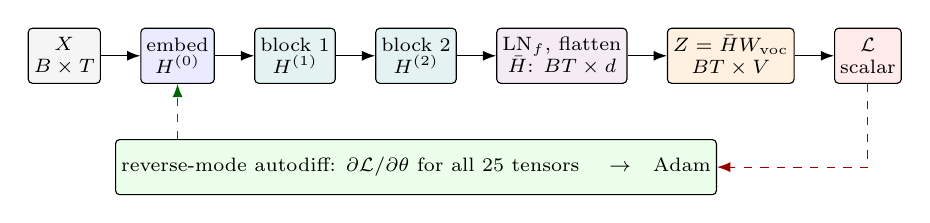
\begin{tikzpicture}[node distance=4mm and 5mm, every node/.style={font=\scriptsize},
  box/.style={draw, rounded corners=1.5pt, fill=#1, minimum height=7mm, align=center, inner sep=2pt}, >=Latex]
\node[box=gray!8] (x) {$X$\\$B\times T$};
\node[box=blue!8, right=of x] (e) {embed\\$H^{(0)}$};
\node[box=teal!10, right=of e] (b1) {block 1\\$H^{(1)}$};
\node[box=teal!10, right=of b1] (b2) {block 2\\$H^{(2)}$};
\node[box=violet!8, right=of b2] (lnf) {$\LN_f$, flatten\\$\Hbar$: $BT\times d$};
\node[box=orange!12, right=of lnf] (z) {$Z=\Hbar\Wvoc$\\$BT\times V$};
\node[box=red!8, right=of z] (l) {$\mathcal L$\\scalar};
\foreach \a/\b in {x/e,e/b1,b1/b2,b2/lnf,lnf/z,z/l} \draw[->] (\a) -- (\b);
\node[box=green!8, below=7mm of b2, minimum width=70mm] (ad) {reverse-mode autodiff: $\partial\mathcal L/\partial\theta$ for all 25 tensors \quad$\to$\quad Adam};
\draw[->, red!60!black, dashed] (l.south) |- (ad.east);
\draw[->, green!40!black, dashed] (ad.north -| e.south) -- (e.south);
\end{tikzpicture}
\captionof{figure}{The complete computation. Solid arrows are the forward pass, dashed arrows the gradient and the update.}
\label{fig:pipeline}
\end{center}

\subsection{What is reused from Assignment 1, and how compatibility was verified}
The Assignment~1 package \code{python/gpt_a1/} and its MATLAB functions are included \emph{unchanged}, so this archive is
self-contained. The new code imports them and never edits them.

\begin{center}
\small
\begin{tabular}{@{}p{4.3cm}p{5.2cm}p{6.2cm}@{}}
\toprule
\textbf{Reused function} & \textbf{Role here} & \textbf{Compatibility evidence}\\ \midrule
\code{Tensor} (autodiff engine) & differentiates the whole GPT & every hand-derived gradient agrees with it to \chkpy{Q3.2} (\code{Q3.2})\\
\code{load_corpus}, \code{build_vocab}, \code{encode}, \code{split_contiguous}, \code{get_batch} & data, split and windows &
identical vocabulary to Assignment~1's saved \code{vocab.json} (\code{D.1})\\
\code{init_params}, \code{count_params} & the 25 tensors, $P=\Ptotal$ & the saved \code{params_init.npz} equals a re-run of
the Assignment~1 initialization (\code{D.2}, \code{D.3}); fixed-input logits agree exactly (\code{D.4})\\
\code{embed}, \code{layer_norm}, \code{softmax_rows}, \code{causal_mask} & inside every block & block-1 attention on a held-out
batch equals the standalone Assignment~1 routine (\code{B5.1}: \BfiveErr)\\
\code{embedding_backward}, \code{layer_norm_backward}, \code{attention_backward} & the hand-derived chain rule & term-by-term
agreement with autodiff through all 25 tensors (\code{Q3.2})\\
\bottomrule
\end{tabular}
\end{center}

\subsection{Code organisation}
\begin{center}
\small
\begin{tabular}{@{}p{4.6cm}p{11.2cm}@{}}
\toprule
\textbf{File} & \textbf{Content}\\ \midrule
\code{python/gpt_a2/ops.py} & the new differentiable primitives \code{tanh}, \code{log}, \code{pick} (target gathering) and GELU composed from them\\
\code{python/gpt_a2/model.py} & attention inside a block, feed-forward network, residual blocks, logits, cross-entropy; hand-derived backward maps\\
\code{python/gpt_a2/optim.py} & Adam from its definition\\
\code{python/gpt_a2/train.py} & step budget, training loop, held-out validation, fixed-window evaluation\\
\code{python/gpt_a2/sample.py} & context cropping and categorical (or greedy) sampling\\
\code{python/run_assignment2.py} & runs Q1--Q6, Benchmark B, Cases B1--B5, the acceptance tests, training and generation; writes \code{results/python/}\\
\code{python/tests/} & 15 unit tests of the new package and 23 of the reused one (standard-library \code{unittest})\\
\code{matlab/src/*.m}, \code{matlab/run_assignment2.m} & the MATLAB twin: one function per operation, the same check ids\\
\code{report/build_assets.py} & turns \code{results/*/results.json} into every table, number and listing of this report\\
\bottomrule
\end{tabular}
\end{center}

\subsection{Conventions}
\begin{itemize}
\item \textbf{Indices.} Python labels are $0,\dots,V-1$; MATLAB labels are $1,\dots,V$. Worked examples print the
mathematical one-based labels.
\item \textbf{Right multiplication.} Every linear map is $Y=XW+\one b$ with $W\in\R^{d_{\rm in}\times d_{\rm out}}$, as in
the assignment; no transposed \code{nn.Linear} convention.
\item \textbf{Flattening order} (Section~\ref{sec:q2}). Python flattens $B\times T\times d$ hidden states and $B\times T$
targets row-major, so row $r=bT+t$ (time-major within each batch member). MATLAB flattens both column-major, so
$r=b+(t-1)B$. Each language uses one rule for \emph{both} hidden states and labels.
\item \textbf{Objective.} $\mathcal L$ is the mean over all $BT$ predicted characters, so the $1/(BT)$ factor appears once,
inside the loss, and never again in a gradient.
\item \textbf{Precision.} IEEE double precision throughout.
\end{itemize}

\subsection{Automatic differentiation: three new local derivatives}
The engine of Assignment~1 records, for every operation, its parents and a closure that applies the local chain rule
$\bar x\mathrel{+}=(\partial y/\partial x)\T\bar y$; \code{backward()} runs the closures in reverse topological order. The
GPT head and the GELU need three more primitives, added through the same hook:
\begin{equation}
d\tanh x=(1-\tanh^2x)\,dx,\qquad d\log x=dx/x,\qquad z_r=Z_{r,y_r}\ \Rightarrow\ \bar Z_{r,y_r}\mathrel{+}=\bar z_r .
\end{equation}
GELU is \emph{not} a primitive: it is composed from \code{tanh}, products and sums, so its derivative comes from the
engine and can be compared with the hand-derived $g'(z)$ (\code{Q1.3}). In MATLAB the same role is played by
\code{dlfeval}/\code{dlgradient} on \code{dlarray} copies of the parameters (\code{dl_gpt_loss.m}).
\lstinputlisting[style=py,caption={Python: the new differentiable primitives (\code{gpt_a2/ops.py}).}]{generated/snippets/py_ops.py}

\subsection{How every derivative is verified}
Each gradient is computed in three independent ways: (i) the hand-derived matrix calculus of this report, written on
plain arrays (\code{*_backward}); (ii) automatic differentiation of the forward code; (iii) centred finite differences
$[\mathcal L(\theta+\delta e_k)-\mathcal L(\theta-\delta e_k)]/(2\delta)$, with the relative discrepancy
$\rho=|a-b|/\max(1,|a|,|b|)$ of the assignment. (i) against (ii) is checked term by term for every intermediate, and
(ii) against (iii) for at least one scalar of every kind of tensor.

\subsection{Departures from the specification and choices it leaves open}
\begin{enumerate}
\item \textbf{Two implementations.} Both are complete and both were run. Python is the reference for the figures and the
worked numbers of this report. \ifnum\MlRun=1 MATLAB passes the same checks under the same ids (Table~\ref{tab:checks}),
trains its own model (Case~B4) and generates its own sample (Section~\ref{sec:q5}).\else The MATLAB program was written
alongside but is not run in the environment that produced this report; it writes \code{results/matlab/} and rebuilding
the report adds its column.\fi
\item \textbf{Own autodiff in Python instead of PyTorch.} For automatic differentiation the assignment names
\code{loss.backward()} in PyTorch or \code{dlfeval} and \code{dlgradient} in MATLAB. The MATLAB program uses \code{dlgradient} exactly as named. The Python program uses the
engine of Assignment~1, which provides the same \code{backward()} interface without a framework; both automatic
gradients are checked against the hand-derived chain rule and against finite differences.
\item \textbf{Integer step budget.} $N_{\rm tr}/(BT)=\Ntr/2048$ is not an integer; $S_{\rm epoch}=\lfloor N_{\rm tr}/(BT)\rfloor=\Sepoch$.
\item \textbf{Starting point.} Training starts from the initialization Assignment~1 saved, not from a new draw (each
language from its own file, \code{params_init.npz} or \code{params_init.mat}): the hand-off is then tested exactly
(\code{D.3}, \code{D.4}, \code{B5.1}).
\item \textbf{Low-noise final estimate.} In addition to the periodic 8-window validation batches, the final losses are
averaged over \NfixedVa{} fixed validation windows whose starts are spread evenly over the held-out part (and likewise
\NfixedTr{} training windows), as the assignment recommends.
\end{enumerate}

% =====================================================================================
\section{Question 1: residual connections and the feed-forward network}\label{sec:q1}

\begin{purpose}[1. Purpose and assumptions]
Attention lets each token read earlier tokens; the feed-forward network (FFN) then transforms each token's features on
its own, with a nonlinearity. Residual sums keep an identity path around both sub-layers, so information and gradients
can pass a block unchanged when the sub-layer contributes little. The block is pre-normalized: each sub-layer sees a
LayerNorm of its input, the residual path does not.
\end{purpose}

\stephead{2. Derivation}
For batch member $b$ and block $\ell$, with $F_b$ the attention output of Assignment~1,
\begin{align}
R_b &= H_b^{(\ell-1)}+F_b, & D_b&=\LN_2(R_b), \\
J_b &= D_bW_1^{(\ell)}+\one_Tb_1^{(\ell)}\in\R^{T\times4d}, & G_b&=g(J_b)\,W_2^{(\ell)}+\one_Tb_2^{(\ell)}\in\R^{T\times d},\qquad
H_b^{(\ell)}=R_b+G_b,
\end{align}
with $W_1\in\R^{d\times4d}$, $b_1\in\R^{1\times4d}$, $W_2\in\R^{4d\times d}$, $b_2\in\R^{1\times d}$. Entry by entry,
\begin{equation}
(J_b)_{ik}=\sum_{j=1}^{d}(D_b)_{ij}(W_1)_{jk}+(b_1)_k,\qquad (G_b)_{ij}=\sum_{k=1}^{4d}g\big((J_b)_{ik}\big)(W_2)_{kj}+(b_2)_j .
\end{equation}
Row $i$ of $G_b$ depends on row $i$ of $D_b$ only: the FFN mixes \emph{features} of one token. Attention instead forms
$A_bV_b$, whose row $i$ is $\sum_{j\le i}A_{ij}V_{j,:}$: it mixes \emph{tokens}. Because no token interacts with another in the
FFN, all $BT$ rows are flattened into one $(BT)\times d$ matrix and multiplied at once.

\textbf{GELU.} The implementation uses the tanh approximation, with $a=\sqrt{2/\pi}$, $c=0.044715$, $u(z)=a(z+cz^3)$,
\begin{equation}
g(z)=\tfrac z2\big(1+\tanh u(z)\big),\qquad g'(z)=\tfrac12\big(1+\tanh u\big)+\tfrac z2\big(1-\tanh^2u\big)\,a\,(1+3cz^2).
\end{equation}
The exact GELU is $z\Phi(z)$ with $\Phi$ the standard normal distribution function.

\textbf{Residual Jacobian.} For $R=H+F(H)$, the differential is $dR=dH+J_F(H)\,dH$, so
\begin{equation}
\frac{\partial R}{\partial H}=I+J_F(H),\qquad
\frac{\partial\mathcal L}{\partial H}=G_R+J_F(H)\T G_R ,
\end{equation}
where $G_R=\partial\mathcal L/\partial R$. The first term reaches $H$ unchanged, however small $J_F$ is; stacking blocks
multiplies factors $(I+J_{F_\ell})$, whose identity parts keep the product from vanishing. This is why residual connections
make deeper stacks trainable.

\textbf{FFN derivatives.} With $\mathcal R=g(J)$ (rows flattened), $G=\mathcal RW_2+\one b_2$ and upstream $G_G$:
\begin{align}
G_{W_2}&=\mathcal R\T G_G, & G_{b_2}&=\one\T G_G, & G_{\mathcal R}&=G_GW_2\T, & G_J&=G_{\mathcal R}\odot g'(J),\\
G_{W_1}&=D\T G_J, & G_{b_1}&=\one\T G_J, & G_D&=G_JW_1\T . \notag
\end{align}
Each bias gradient is a sum over all $BT$ rows because the same bias row is added to every row. Through the two residual
sums, $G_R=G_{H'}+\big(\text{LN}_2\text{-backward of }G_D\big)$ and $G_H=G_R+\big(\text{LN}_1\text{-backward of the attention input gradient}\big)$.

\stephead{3. Code}
\lstinputlisting[style=py,caption={Python: the feed-forward network and the residual block (\code{gpt_a2/model.py}).}]{generated/snippets/py_ffn.py}
\lstinputlisting[style=py,caption={Python: attention as it runs inside a block (batched over the leading axis).}]{generated/snippets/py_attention.py}
\lstinputlisting[style=ml,caption={MATLAB: \code{ffn_forward.m}.}]{generated/snippets/ffn_forward.m}
\lstinputlisting[style=ml,caption={MATLAB: \code{block_forward.m}.}]{generated/snippets/block_forward.m}
\lstinputlisting[style=py,caption={Python: the hand-derived FFN backward map and $g'$.}]{generated/snippets/py_ffn_back.py}
\lstinputlisting[style=py]{generated/snippets/py_gelu_grad.py}
\lstinputlisting[style=ml,caption={MATLAB: \code{ffn_backward.m} and \code{block_backward.m}.}]{generated/snippets/ffn_backward.m}
\lstinputlisting[style=ml]{generated/snippets/block_backward.m}

\stephead{4. Operation-by-operation explanation}
\begin{ops}
\code{D.reshape(B * T, d) @ W_1 + b_1} & \code{reshape(D, B*T, d) * W_1 + b_1} & $J$: $(BT\times d)(d\times4d)$; the
$1\times4d$ bias row is broadcast (implicit expansion) to every row\\
\code{ops.gelu(J)} & \code{gelu_tanh(J)} & elementwise $g$; $(BT)\times4d$\\
\code{(Ga @ W_2 + b_2).reshape(B, T, d)} & \code{reshape(Ga * W_2 + b_2, B, T, d)} & $G$: $(BT\times4d)(4d\times d)$, back to
$B\times T\times d$\\
\code{R = H + F}; \code{Hn = R + G} & \code{R = H + F;} \code{Hn = R + G;} & the two residual sums, $B\times T\times d$\\
\code{Ga.T @ G2}; \code{G2.sum(axis=0)} & \code{cache.Ga' * G2}; \code{sum(G2, 1)} & $G_{W_2}$ ($4d\times d$), $G_{b_2}$ ($1\times d$)\\
\code{G_Ga * ops.gelu_grad_np(J)} & \code{g.Ga .* gelu_grad(cache.J)} & $G_J=G_{\mathcal R}\odot g'(J)$\\
\code{G_R = G_Hn + G_R_ln} & \code{G_R = G_Hn + G_R_ln;} & identity path plus branch: $\partial\mathcal L/\partial R$\\
\end{ops}

\stephead{5. Numerical verification and interpretation}
\textbf{The small case $d=2$.} With $W_1\in\R^{2\times8}$, $b_1\in\R^{1\times8}$, $W_2\in\R^{8\times2}$, $b_2\in\R^{1\times2}$,
the self-chosen token row $D=(0.5,\,-1)$, $b_2=(0.05,\,-0.05)$ and
{\setlength{\arraycolsep}{3pt}
\[
W_1=\SmallWone,\qquad b_1=\SmallBone,
\]
the elementwise sums give
\begin{gather*}
J=\SmallJ,\\
g(J)=\SmallgJ,\\
G=\SmallG .
\end{gather*}}
identical to the vectorized code within \chkpy{Q1.1} (\code{Q1.1}). Negative entries of $J$ are damped towards zero, not cut
off as in a ReLU.

\textbf{Approximation against the exact GELU} (analytical comparison; the implementation uses the approximation):
\begin{center}
\small
\begin{tabular}{@{}cccc@{}}
\toprule
$z$ & tanh approximation $g(z)$ & exact $z\Phi(z)$ & difference\\ \midrule
$-1$ & \GeluApproxM & \GeluExactM & \GeluDiff\\
$0$ & $0$ & $0$ & $0$\\
$+1$ & \GeluApproxP & \GeluExactP & \GeluDiff\\
\bottomrule
\end{tabular}
\end{center}
The largest difference on $[-6,6]$ is \GeluGridMax. The hand-derived $g'$ agrees with the engine's derivative of the composed
GELU within \GeluGradAuto{} on 2401 points (\code{Q1.3}) and with centred differences within \GeluGradFD.

\begin{figure}[!htb]
\centering
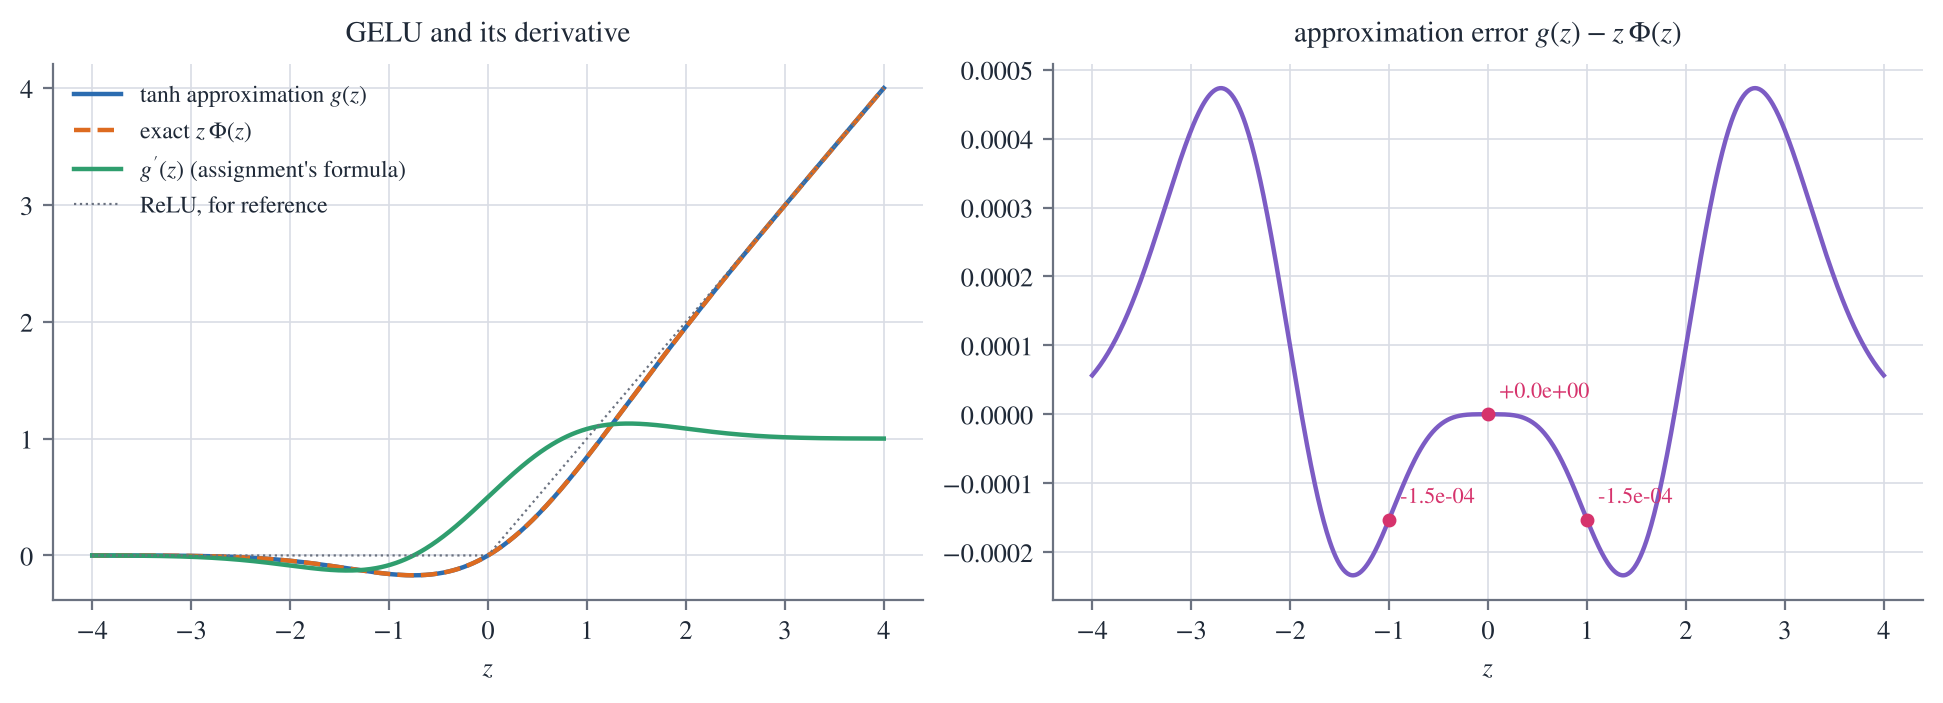
\includegraphics[width=0.92\linewidth]{gelu.png}
\caption{Left: the tanh-GELU, the exact GELU and $g'$. Right: the approximation error, $\approx1.5\times10^{-4}$ at $z=\pm1$.}
\label{fig:gelu}
\end{figure}

\textbf{The identity path, measured.} For one block with $T=4$, $d=3$, the full $12\times12$ Jacobians of $R$ and of $F$ with
respect to $H$ were formed by centred differences; $\partial R/\partial H-J_F-I$ is at most \ResJacErr{} (\code{Q1.4}). The
token-by-token maxima show the two kinds of mixing:
\[
\Big[\max\Big|\frac{\partial F_i}{\partial H_j}\Big|\Big]_{ij} = \BlockF ,
\]
\[
\Big[\max|\Delta G_i|\text{ after changing }D_j\Big]_{ij} = \BlockG .
\]
Attention is lower triangular in tokens (rows $i$, columns $j$; exactly $0$ above the diagonal, \code{Q1.6}); the FFN is
diagonal, exactly $0$ off the diagonal (\code{Q1.5}). Every term of the FFN backward map matches automatic
differentiation within \FFNTermsErr{} (\code{Q1.7}).

\begin{result}[Case B2: random feed-forward and residual (seed 451, $B=2$, $T=5$, $d=4$, $d_{\rm ff}=16$)]
$H$, $W_1$, $W_2$ have $\mathcal N(0,0.02^2)$ entries, biases are $0$, gains are $1$. Per sample, $J\in\R^{5\times16}$,
$G\in\R^{5\times4}$, $H_{\rm next}=H+G\in\R^{5\times4}$ (\code{B2.1}, \code{B2.2}). For $\mathcal J=\sum_{b,i,j}(H_{\rm next})_{bij}^2$,
centred differences on five random entries of $W_1$ and five of $W_2$ give:
\begin{center}
\small
\begin{tabular}{@{}lccccc@{}}
\toprule
entry & autodiff & $h=10^{-3}$ & $10^{-4}$ & $10^{-5}$ & $10^{-6}$\\ \midrule
\tabinput{generated/tab_b2.tex}
\bottomrule
\end{tabular}
\end{center}
Because the objective is quadratic in $W_2$ and smooth in $W_1$, truncation error is negligible; with weights of size
$0.02$ the derivatives are $\sim10^{-4}$, so the step $h=10^{-5}$ keeps the perturbation small relative to the weights while
the round-off error $\approx\varepsilon_{\rm mach}\mathcal J/h$ stays near $10^{-12}$. Worst error at $h=10^{-5}$: \BtwoRel{}
(assignment measure, \code{B2.3}); scale-free relative error \BtwoStrict{} (\code{B2.4}).
\end{result}

% =====================================================================================
\section{Question 2: vocabulary projection and cross-entropy}\label{sec:q2}

\begin{purpose}[1. Purpose and assumptions]
The last hidden state of each position must become a probability distribution over the $V$ characters, and training needs
one scalar that rewards probability on the actual next character. Logits are unrestricted scores; probabilities are their
softmax; the loss is the mean negative log-probability of the targets, computed without ever forming a probability that
could underflow.
\end{purpose}

\stephead{2. Derivation}
After the final normalization, the $B$ matrices $\LN_f(H_b^{(L)})\in\R^{T\times d}$ are flattened into $\Hbar\in\R^{BT\times d}$
and projected:
\begin{equation}
\underbrace{\Hbar}_{BT\times d}\ \underbrace{\Wvoc}_{d\times V}=\underbrace{Z}_{BT\times V} .
\end{equation}
The targets $Y$ are flattened into $(y_1,\dots,y_{BT})$ by the same rule, so row $r$ of $Z$ is scored against $y_r$. With
$a_r=\max_jZ_{rj}$,
\begin{equation}
\LSE_r=a_r+\log\sum_{j=1}^Ve^{Z_{rj}-a_r},\qquad
\mathcal L=-\frac1{BT}\sum_{r=1}^{BT}\big(Z_{r,y_r}-\LSE_r\big),\qquad p_{rj}=e^{Z_{rj}-\LSE_r}.
\end{equation}
\textbf{Why the shift changes nothing.} For any constant $c_r$, $\softmax(Z_{r,:}+c_r)=\softmax(Z_{r,:})$ and
$\LSE(Z_{r,:}+c_r)-(Z_{r,y_r}+c_r)=\LSE(Z_{r,:})-Z_{r,y_r}$. Choosing $c_r=-a_r$ makes every exponent $\le0$ (no overflow) and
one exponent equal to $0$ (the sum is $\ge1$, so its logarithm is finite).

\textbf{Gradient.} The softmax Jacobian of one row is $\partial p_i/\partial z_j=p_i(\delta_{ij}-p_j)$. For one row,
$\ell=\LSE(z)-z_y$, so $\partial\ell/\partial z_j=p_j-\mathbb 1[j=y]$. Averaging over the $BT$ rows, with $E$ the one-hot
targets,
\begin{equation}
\frac{\partial\mathcal L}{\partial Z}=\frac{P-E}{BT}\in\R^{BT\times V},\qquad
\frac{\partial\mathcal L}{\partial\Wvoc}=\Hbar\T\frac{P-E}{BT}\in\R^{d\times V},\qquad
\frac{\partial\mathcal L}{\partial\Hbar}=\frac{P-E}{BT}\Wvoc\T\in\R^{BT\times d}.
\end{equation}
Each row of $P-E$ sums to $\sum_jp_{rj}-1=0$. \textbf{Uniform logits.} If $Z=0$, then $p_{rj}=1/V$ and every term is
$-\log(1/V)$, so $\mathcal L=\log V=\logV$ for $V=\Vsize$: the loss of a model that knows nothing. A target probability of
$0.7$ contributes $-\log0.7\approx0.357$.

\stephead{3. Code}
\lstinputlisting[style=py,caption={Python: the complete forward pass, the cross-entropy and the training objective (\code{gpt_a2/model.py}).}]{generated/snippets/py_gpt.py}
\lstinputlisting[style=py,caption={Python: $\partial\mathcal L/\partial Z=(P-E)/R$.}]{generated/snippets/py_ce_back.py}
\lstinputlisting[style=ml,caption={MATLAB: \code{gpt_forward.m} and \code{cross_entropy.m}.}]{generated/snippets/gpt_forward.m}
\lstinputlisting[style=ml]{generated/snippets/cross_entropy.m}

\stephead{4. Operation-by-operation explanation}
\begin{ops}
\code{Hf.reshape(B * T, d)} & \code{reshape(Hf, B*T, d)} & $\Hbar$; Python row $r=bT+t$, MATLAB row $r=b+(t-1)B$\\
\code{Hbar @ P["W_voc"]} & \code{Hbar * P.W_voc} & $Z$: $(BT\times d)(d\times V)$\\
\code{Z.max(axis=1, keepdims=True)} & \code{max(Z, [], 2)} & $a_r$, $BT\times1$; a constant shift\\
\code{a + ops.log((Z - a).exp().sum(axis=1, keepdims=True))} & \code{a + log(sum(exp(Z - a), 2))} & $\LSE_r$; every exponent $\le0$\\
\code{ops.pick(Z, y)} & \code{Z(sub2ind(size(Z), (1:R)', y(:)))} & $Z_{r,y_r}$ for all rows at once (no loop)\\
\code{(lse - picked).mean()} & \code{mean(lse - Z(idx))} & $\mathcal L$, the mean over $BT$ rows\\
\code{G[np.arange(R), y] -= 1; G / R} & \code{G(idx) = G(idx) - 1; G / R} & $(P-E)/(BT)$\\
\end{ops}

\stephead{5. Numerical verification and interpretation}
\textbf{The $2\times3$ example.} For $Z=\begin{bmatrix}2&0&-1\\0&1&0\end{bmatrix}$ and one-based labels $y=(1,2)$: the row maxima
are $a=(2,1)$, $\LSE_1=\log(e^2+1+e^{-1})=\CEexLSEa$, $\LSE_2=\log(2+e)=\CEexLSEb$, the negative log-likelihoods are
$\LSE_1-2=\CEexNLLa$ and $\LSE_2-1=\CEexNLLb$, and
\[
\mathcal L=\tfrac12\big[\log(e^2+1+e^{-1})-2+\log(2+e)-1\big]=\CEexL\quad(\text{closed form }\CEexRef),
\]
\[
\frac{\partial\mathcal L}{\partial Z}=\frac{P-E}{2}=\CEexGrad .
\]
Both rows of the gradient sum to zero and agree with autodiff (\code{Q2.2}). Adding $(+1000,-1000)$ to the two rows leaves the
stable loss at \ShiftStable{}; without the shift the computation returns \ShiftNaive{} (\code{Q2.3}).

\textbf{The ordering requirement.} For the label matrix $\begin{bmatrix}1&2&3\\4&5&6\end{bmatrix}$, Python's row-major
flattening gives \OrdPy, MATLAB's \code{Y(:)} gives \OrdMl. On a random $2\times3\times4$ batch, flattening hidden states and
labels with the same rule gives the same mean loss in either language (row-major \LOrdPy, column-major \LOrdMl), and a joint
random permutation of rows and labels does too (\LOrdPerm; \code{Q2.4}). Pairing row-major hidden states with
column-major labels instead gives \LOrdMix: wrong targets for four of six rows (\code{Q2.5}). The rule used everywhere in
this submission is therefore fixed per language and applied to both arrays in the same line of code.

\begin{result}[Case B1: fixed logit matrix and exact cross-entropy]
For $Z=\begin{bmatrix}0&0&0\\\log2&0&0\\0&\log3&0\end{bmatrix}$ and $y=(1,1,2)$,
\[
P=\BoneP,
\]
\[
\frac{\partial\mathcal L}{\partial Z}=\frac{P-E}3=\BoneGrad .
\]
The correct-class probabilities are $1/3$, $1/2$ and $3/5$ (\code{B1.3}), so
$\mathcal L=\tfrac13\big(\log3+\log2+\log\tfrac53\big)=\BoneRef$; the program measures \BoneL{} (\code{B1.1}, error
\chkpy{B1.1}) and the gradient error is \chkpy{B1.2} (\code{B1.2}). Adding $(5,-3,100)$ to the three rows changes the loss by
\chkpy{B1.4}: a constant shift of a row changes neither its probabilities nor its loss.
\end{result}

% =====================================================================================
\section{Question 3: automatic differentiation and Adam}\label{sec:q3}

\begin{purpose}[1. Purpose and assumptions]
Training needs $\nabla_\theta\mathcal L$ for all 25 tensors at every step. Automatic differentiation evaluates the chain
rule through the computational graph the forward code actually builds. Adam then turns each gradient into an update whose
size is normalized per coordinate. Computing the gradient and applying the update are separate steps: the first only
reads the parameters, the second only changes them.
\end{purpose}

\stephead{2. Derivation}
\textbf{The gradient flow.}
\begin{equation}
\mathcal L\longrightarrow Z\longrightarrow\Hbar\longrightarrow\big(H^{(L)},\dots,H^{(0)}\big)\longrightarrow(W_E,W_P).
\end{equation}
The edge $\mathcal L\to Z$ carries $(P-E)/(BT)$; $Z\to\Hbar$ meets $\Wvoc$ (gradient $\Hbar\T\partial\mathcal L/\partial Z$,
$d\times V$); $\Hbar\to H^{(L)}$ meets $\gamma_f,\beta_f$; each block $\ell$ meets $W_1,b_1,W_2,b_2,\gamma_2,\beta_2$ on its FFN
branch and $W_{QKV},W_O,\gamma_1,\beta_1$ on its attention branch, while the residual identity carries the gradient past both;
$H^{(0)}\to(W_E,W_P)$ gives $\partial\mathcal L/\partial W_E=\sum_bO_b\T G_{H_b}$ and
$\partial\mathcal L/\partial W_P[t,:]=\sum_bG_{H_b}[t,:]$. Only the rows of $W_E$ whose characters occur in the batch receive
a gradient; on the real batch below, \WErowsHit{} of the $V=\Vsize$ rows do.

\textbf{Why the embeddings must stay in the graph.} If $W_E$ entered the forward pass as a numerical copy without history,
the chain would stop at $H^{(0)}$: no gradient would reach $W_E$, Adam would never move it, and the model could not learn
which character is which (\code{Q3.6}).

\textbf{Adam.} For the gradient $g_t$ at step $t$,
\begin{gather}
m_t=\beta_1m_{t-1}+(1-\beta_1)g_t,\qquad v_t=\beta_2v_{t-1}+(1-\beta_2)g_t\odot g_t,\\
\hat m_t=\frac{m_t}{1-\beta_1^t},\qquad\hat v_t=\frac{v_t}{1-\beta_2^t},\qquad
\theta_t=\theta_{t-1}-\eta\frac{\hat m_t}{\sqrt{\hat v_t}+\epsilon_A}.
\end{gather}
Because $m_0=v_0=0$, the raw moments are biased towards zero in early steps; dividing by $1-\beta^t$ removes that bias. At
$t=1$, $\hat m_1=g_1$ and $\hat v_1=g_1^2$, so $\theta_1-\theta_0=-\eta\,g_1/(|g_1|+\epsilon_A)\approx-\eta\operatorname{sign}(g_1)$.

\textbf{Numerical exercise} ($g_1=0.2$, $\beta_1=0.9$, $\beta_2=0.999$, $\eta=0.001$, $\epsilon_A=10^{-8}$):
$m_1=0.1\cdot0.2=\AdamMone$, $v_1=0.001\cdot0.04=\AdamVone$, $\hat m_1=\AdamMhat$, $\hat v_1=\AdamVhat$, and the first update is
$-0.001\cdot0.2/(0.2+10^{-8})=\AdamUpd$ (\code{Q3.1}).

\stephead{3. Code}
\lstinputlisting[style=py,caption={Python: the hand-derived backward pass through a block and through the whole GPT (\code{gpt_a2/model.py}).}]{generated/snippets/py_block_back.py}
\lstinputlisting[style=py,caption={Python: Adam (\code{gpt_a2/optim.py}).}]{generated/snippets/py_adam.py}
\lstinputlisting[style=ml,caption={MATLAB: \code{gpt_backward.m}, the traced objective \code{dl_gpt_loss.m}, and \code{adam_step.m}.}]{generated/snippets/gpt_backward.m}
\lstinputlisting[style=ml]{generated/snippets/dl_gpt_loss.m}
\lstinputlisting[style=ml]{generated/snippets/adam_step.m}

\stephead{4. Operation-by-operation explanation}
\begin{ops}
\code{L_t.backward()} & \code{dlfeval(@dl_gpt_loss, ...)} & every $\partial\mathcal L/\partial\theta$ by reverse-mode autodiff\\
\code{Hbar.T @ G_Z} & \code{c.Hbar' * G_Z} & $\partial\mathcal L/\partial\Wvoc$, $(d\times BT)(BT\times V)=d\times V$\\
\code{(G_Z @ W_voc.T).reshape(B, T, d)} & \code{reshape(G_Z * P.W_voc', c.B, c.T, d)} & undo the flattening with the same rule\\
\code{for l in range(L, 0, -1)} & \code{for l = nb:-1:1} & blocks in reverse order\\
\code{A1.embedding_backward(G_H, O, T_max)} & \code{embed_backward(G_H, c.O, ...)} & $\sum_bO_b\T G_{H_b}$ and $\sum_bG_{H_b}$\\
\code{self.m[k] = b1 * self.m[k] + (1 - b1) * g} & \code{state.m.(n) = beta1 * state.m.(n) + ...} & first moment\\
\code{m_hat / (np.sqrt(v_hat) + self.eps)} & \code{(m / c1) ./ (sqrt(v / c2) + eps_a)} & bias-corrected, per-coordinate step\\
\code{theta += delta} & \code{F.(n) = F.(n) + step} & the update (in place in Python)\\
\end{ops}

\stephead{5. Numerical verification and interpretation}
On a real batch ($B=32$, $T=64$) at the Assignment~1 initialization (loss \FullLoss), the hand-derived chain rule and the
autodiff engine agree for every one of the 25 tensors to \FullErr{} (\code{Q3.2}); none of the tensors has an all-zero
gradient, so every parameter lies on a path from $\mathcal L$ (\code{Q3.3}); $\partial\mathcal L/\partial\Wvoc=\Hbar\T\partial\mathcal L/\partial Z$
has shape $d\times V=64\times\Vsize$ and matches (\code{Q3.4}); the gradients of $W_E$ and $W_P$ are finite and non-zero
(\code{Q3.5}). With $W_E$ replaced by a detached copy, no gradient reaches $W_E$ while $W_P$ still receives one (\code{Q3.6}).

\begin{result}[Case B3, part 1: one Adam step on a random $2\times3$ matrix (seed 451)]
\[
\theta_0=\BthreeThetaZero,\qquad g=\BthreeG,
\]
\[
m_1=\BthreeM,\qquad v_1=\BthreeV,
\]
\[
\theta_1=\BthreeThetaOne .
\]
The optimizer and the matrix equations agree to \BthreeErr{} (\code{B3.1}). Every entry moved by almost exactly
$-\eta\operatorname{sign}(g)$: at $t=1$ Adam ignores the size of the gradient and keeps only its direction.
\end{result}

% =====================================================================================
\section{Required Benchmark B: deterministic logits, loss, gradients and Adam}\label{sec:bench}

\begin{purpose}[Setup and prediction]
$B=1$, $T=2$, $d=2$, $V=3$. Residual test: $H=I_2$, attention output $F=0$, $W_1=W_2=0$, $b_1=b_2=0$, so $R=H$, the FFN output
is $0$ and $H'=H$. Head test: $\Hbar=I_2$ supplied directly, $\Wvoc=0_{2\times3}$, one-based targets $(y_1,y_2)=(2,3)$.
\end{purpose}
Measured: $R=H$, $G=0$, $H'=H$ exactly (\code{BB.1}). The logits are $Z=0$, every probability is $1/3$, and
\[
P=\BenchP,\qquad \mathcal L=\BenchL=\log3,
\]
\[
\frac{\partial\mathcal L}{\partial Z}=\frac{P-E}2=\BenchGZ,\qquad
\frac{\partial\mathcal L}{\partial\Wvoc}=\Hbar\T\frac{P-E}2=\BenchGW ,
\]
all within \chkpy{BB.3} of the displayed values (\code{BB.2}, \code{BB.3}). The first Adam step gives
\[
\Wvoc^{\rm new}=\BenchWnew ,
\]
equal to $-\eta g/(|g|+\epsilon_A)$ within \chkpy{BB.4} and to the rounded display $\pm0.001$ within \chkpy{BB.5}
(\code{BB.4}, \code{BB.5}).

\textbf{Why zero weights give uniform probabilities but a non-zero gradient.} $\Wvoc=0$ makes every logit $0$, hence
$P=\tfrac13\one\one\T$ whatever $\Hbar$ is. The gradient $\Hbar\T(P-E)/2$, however, depends on $\Hbar$ and on the targets:
$P-E$ is non-zero because the targets are one-hot and the prediction is not. The gradient points from the uniform guess
towards the targets, which is exactly what the first update starts to do.

% =====================================================================================
\section{Question 4: training schedule, validation and gradient checks}\label{sec:q4}

\begin{purpose}[1. Purpose and assumptions]
Training repeats: draw fresh windows from the training part, compute the loss and its gradient, update. Validation measures
the same loss on held-out text, never updating anything. The step budget is defined by the assignment as 50 ``epochs'' of
$S_{\rm epoch}$ steps.
\end{purpose}

\stephead{2. Derivation}
One step consumes $B$ windows of $T$ predictions, i.e.\ $BT$ predicted characters. The step budget is
\begin{equation}
S_{\rm epoch}=\Big\lfloor\frac{N_{\rm tr}}{BT}\Big\rfloor=\Big\lfloor\frac{\Ntr}{2048}\Big\rfloor=\Sepoch,\qquad
S_{\rm total}=50\,S_{\rm epoch}=\StotalFull .
\end{equation}
It is a \emph{budget}, not a pass over the data: the $S_{\rm epoch}B$ starts of one epoch are drawn independently and
uniformly from $M=N_{\rm tr}-T$ possibilities, so some characters are predicted several times and others not at all. A given
character is a target of the $T$ windows that start in the $T$ positions before it, so it is never predicted in an epoch with
probability $(1-T/M)^{S_{\rm epoch}B}\approx\exp(-S_{\rm epoch}BT/M)\approx e^{-1}\approx37\%$. Over 50 epochs that falls to
$e^{-50}$: every character is seen many times, in many different windows.

\textbf{Training loss vs validation loss.} The training loss of step $t$ is computed \emph{before} its update, on the
batch that produces the gradient; it is the quantity being minimized. The validation loss at step $t$ is computed
\emph{after} the update, on 8 fresh windows from the held-out part, with constant parameters: no graph, no gradient, no
change to the Adam moments. Eight windows are only $512$ correlated predictions from a random place in the held-out
text, so each validation value is a noisy estimate: over the last 100 evaluations of the run, the per-evaluation noise,
estimated from the differences of consecutive values (the model barely changes in 50 steps), has a standard deviation of
\ValNoise{} nats. The final
numbers therefore average over \NfixedVa{} fixed windows.

\textbf{Gradient check.} For one scalar $\theta_k$ of each kind of tensor and an identical fixed batch,
\begin{equation}
g_k^{\rm FD}=\frac{\mathcal L(\theta+\delta e_k)-\mathcal L(\theta-\delta e_k)}{2\delta},\qquad
\rho_k=\frac{|g_k^{\rm AD}-g_k^{\rm FD}|}{\max(1,|g_k^{\rm AD}|,|g_k^{\rm FD}|)} .
\end{equation}
The truncation error is $\tfrac{\delta^2}6|\mathcal L'''|$; the round-off error is $\approx\varepsilon_{\rm mach}|\mathcal L|/\delta$
with $\varepsilon_{\rm mach}\approx2.2\times10^{-16}$ and $|\mathcal L|\approx4$. They balance near
$\delta\approx(3\varepsilon_{\rm mach}|\mathcal L|/|\mathcal L'''|)^{1/3}\approx10^{-5}$, which is the step used.

\stephead{3. Code}
\lstinputlisting[style=py,caption={Python: the step budget and the evaluation helpers (\code{gpt_a2/train.py}).}]{generated/snippets/py_schedule.py}
\lstinputlisting[style=py,caption={Python: the training loop.}]{generated/snippets/py_train.py}
\lstinputlisting[style=ml,caption={MATLAB: \code{train_gpt.m} and \code{sample_batch.m}.}]{generated/snippets/train_gpt.m}
\lstinputlisting[style=ml]{generated/snippets/sample_batch.m}

\stephead{4. Operation-by-operation explanation}
\begin{ops}
\code{get_batch(train_ids, B, T, rng_train)} & \code{sample_batch(train, B, T, streams.train)} & fresh windows from the training part only\\
\code{train_curve[s - 1] = float(L_t.data)} & \code{train_curve(s) = Ls;} & loss recorded before the update\\
\code{opt.step(arrays, g)} & \code{adam_step(F, G, state, ...)} & one Adam update of all 25 tensors\\
\code{get_batch(val_ids, B_val, T, rng_val)} & \code{sample_batch(val, B_val, T, streams.val)} & 8 held-out windows, separate generator\\
\code{evaluate(P, Xv, Yv, L)} & \code{cross_entropy(} \code{gpt_forward(...),} \code{Yv(:))} & validation loss on constants: no graph, no update\\
\code{opt.fingerprint() == before} & \code{isequal(before,} \code{adam_fingerprint(state))} & proves the Adam state is unchanged by validation\\
\end{ops}

\stephead{5. Numerical verification and interpretation}
\textbf{Gradient check of the full model} (fixed batch $B=4$, $T=64$, Assignment~1 initialization; the scalar with the
largest gradient in each tensor):
\begin{center}
\small
\setlength{\tabcolsep}{4pt}
\begin{tabular}{@{}lcccccccc@{}}
\toprule
tensor & autodiff & $\delta=10^{-2}$ & $10^{-3}$ & $10^{-4}$ & $10^{-5}$ & $10^{-6}$ & $10^{-7}$ & $10^{-8}$\\ \midrule
\tabinput{generated/tab_fd.tex}
\bottomrule
\end{tabular}
\captionof{table}{$\rho_k$ for one scalar of twelve tensors and seven steps $\delta$.}\label{tab:fd}
\end{center}
The error falls by $10^2$ per decade of $\delta$ down to $\delta=10^{-5}$ (truncation, slope 2) and rises again below it
(round-off): the best step is $\delta=\FDbestDelta$ with worst $\rho=\FDbest$ (\code{Q4.2}, \code{Q4.3}). Every parameter and
gradient is finite (\code{Q4.4}).

\begin{figure}[!htb]
\centering
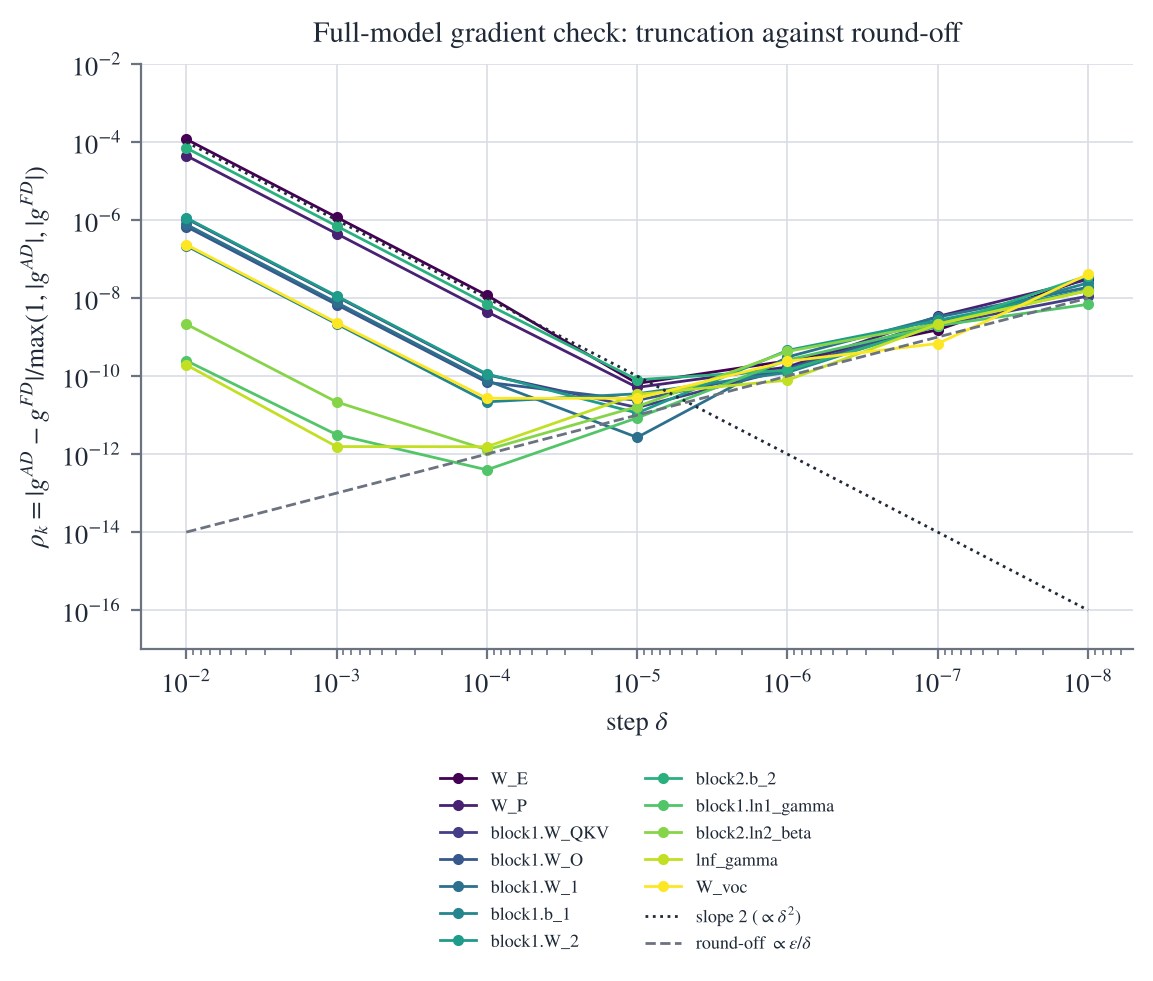
\includegraphics[width=0.62\linewidth]{fd_delta.png}
\caption{Truncation against round-off in the full-model gradient check.}
\label{fig:fd}
\end{figure}

\begin{result}[Case B3, part 2: the complete model on ABAB\dots]
The full architecture ($L=2$, $d=32$, $T=32$, $B=16$, $V=2$) was trained for \SynSteps{} steps on the repeated sequence
\code{ABAB...}. The training loss falls from \SynFirst{} ($\log2=0.6931$) to \SynLast{} (\code{B3.2}); the held-out loss is \SynVal.
Every gradient stayed finite. Samples from the prompt \code{A}:
\VerbatimInput{generated/synthetic.txt}
The greedy continuation never breaks the alternation (\code{B3.3}). This shows that the optimizer and the gradients work end
to end, but not that the model generalizes: the validation text here is the same two-letter pattern, so a falling
training loss proves fitting, not understanding of unseen structure. Generalization is measured on Tiny Shakespeare, below.
\end{result}

\subsection*{Case B4: Tiny Shakespeare end to end}
\addcontentsline{toc}{subsection}{Case B4: Tiny Shakespeare end to end}
Corpus \code{tiny_shakespeare.txt}, SHA-256 {\small\texttt{\expandafter\seqsplit\expandafter{\ShasumFull}}},
$N=\Ncorpus$, $V=\Vsize$; the first $\lfloor0.9N\rfloor=\Ntr$
characters train, the remaining \Nva{} validate; Assignment~1's vocabulary and split are reused, with windows drawn separately
inside each part. Configuration: $B=32$, $T=64$, $d=64$, $L=2$, $\eta=10^{-3}$, \Stotal{} steps (\EpochsRun{} epochs),
evaluation every 50 steps, training seed 451. Training took \TrainMinutes{} minutes on a CPU (NumPy, double precision; the
platform is listed in the reproducibility table at the start).

\begin{figure}[!htb]
\centering
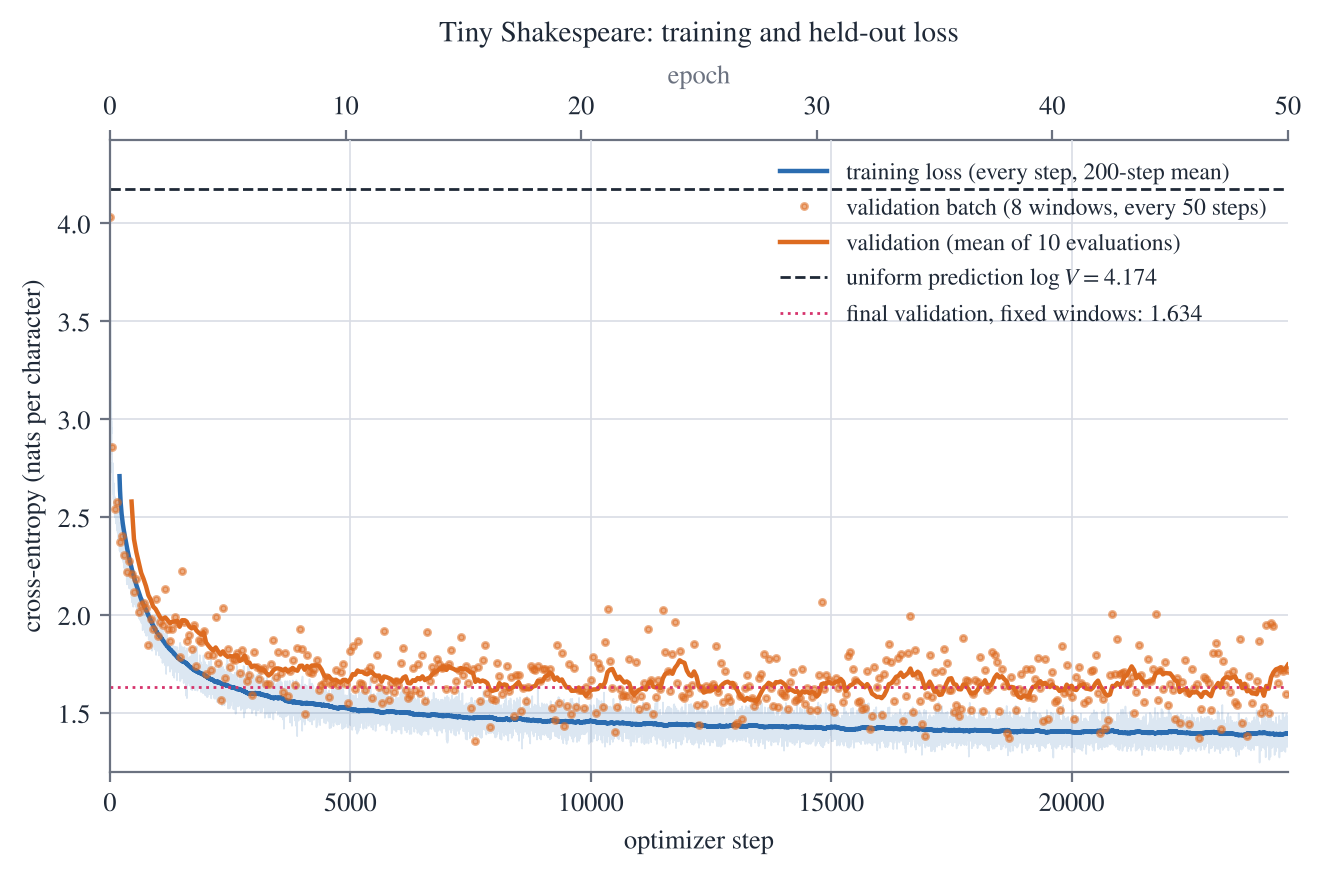
\includegraphics[width=0.95\linewidth]{loss_curves.png}
\caption{Cross-entropy against optimizer step. Blue: training loss of every step (faint) and its 200-step mean; orange: the
8-window validation batches and their running mean; dashed: the uniform level $\log V$; dotted: the final fixed-window
validation loss.}
\label{fig:loss}
\end{figure}

\begin{center}
\small
\begin{tabular}{@{}lcc@{}}
\toprule
& cross-entropy (nats/char) & perplexity $e^{\mathcal L}$\\ \midrule
uniform prediction, $\log V$ & \logV & \Vsize\\
initial model, \NfixedVa{} fixed validation windows & \Lvalinit & \PerplexityInit\\
\textbf{trained, \NfixedVa{} fixed validation windows} & \textbf{\Lvalfixed} & \textbf{\Perplexity}\\
trained, \NfixedTr{} fixed training windows & \Ltrainfixed & \\
generalization gap (validation $-$ training) & \Lgap & \\
\bottomrule
\end{tabular}
\end{center}
The first evaluation (step 1) reads \FirstTrain{} / \FirstVal{} (train / validation batch) and the last \LastTrain{} /
\LastVal. The trained model needs \BitsPerChar{} bits per character on held-out text, against $\log_2V=6.02$ for a uniform
guess. Every validation batch came from the held-out part only and no evaluation changed the optimizer state (\code{B4.2});
exactly $S_{\rm total}$ Adam steps were taken (\code{B4.1}).

\textbf{Interpretation.} The steep drop of the first $\sim$1\,000 steps (two epochs) captures the short-range statistics:
letter frequencies, common pairs and triples of letters, spaces and line breaks. The slow decline afterwards is the model
learning words, speaker tags and punctuation inside its 64-character window.

\textbf{The generalization gap is not small.} On the fixed windows the trained model scores \Lvalfixed{} on held-out text
and \Ltrainfixed{} on training text, a gap of \Lgap{} nats, and Figure~\ref{fig:loss} shows how it builds up. The two curves
separate within the first few epochs, when every training character has been a target only a few times and a model
with $112\,000$ parameters cannot have memorized a million of them. That early part of the gap is a property of the split:
the held-out tenth of the file is the end of \emph{The Taming of the Shrew} and the opening of \emph{The Tempest}, whose
speakers (Prospero, Miranda, Ariel, \dots) never speak in the training part, so it is harder text for any model trained
on the rest (Assignment~1, Section~3). From about epoch 20 on, the validation curve is flat within the noise of its
8-window batches while the training loss keeps falling slowly, so the gap widens towards the end: the late epochs fit the
training plays a little better without transferring to new ones. A run aiming at the lowest held-out loss would stop
earlier or add regularization (dropout, weight decay); this experiment keeps the prescribed 50-epoch budget and reports
the final model.

\ifnum\MlRun=1
\textbf{The same experiment in MATLAB.} \code{run_assignment2.m} trains its own model with the same configuration, the
same schedule ($S_{\rm total}=\MlStotal$ steps), the same evaluation protocol (8-window validation batches at step 1 and every
50 steps, \NfixedVa{} fixed windows per split chosen by the same rule) and gradients from \code{dlfeval}/\code{dlgradient}.
It starts from MATLAB's own saved Assignment~1 initialization (\code{params_init.mat}, drawn with MATLAB's generator, so
its numbers differ from Python's) and draws its windows from MATLAB's Mersenne-Twister streams (seeds 451, 452, 453). It is
therefore a second, independent run of the experiment, not a copy of the Python run:
\begin{center}
\small
\begin{tabular}{@{}lcc@{}}
\toprule
fixed-window cross-entropy (nats/char) & Python (own autodiff) & MATLAB (\texttt{dlgradient})\\ \midrule
held-out text, initial model & \Lvalinit & \MlLvalinit\\
held-out text, trained model & \Lvalfixed & \MlLvalfixed\\
training text, trained model & \Ltrainfixed & \MlLtrainfixed\\
generalization gap & \Lgap & \MlLgap\\
held-out perplexity $e^{\mathcal L}$ & \Perplexity & \MlPerplexity\\
training time (minutes) & \TrainMinutes & \MlMinutes\\
\bottomrule
\end{tabular}
\end{center}
Although it starts from different initial weights and sees different random windows, the MATLAB run ends within
\MlValDiff{} nats of the Python run on held-out text and with practically the same generalization gap, and its curves
(Figure~\ref{fig:lossml}) have the same shape: a steep drop in the first two epochs, then a slowly falling training loss
while the noisy validation batches stay level. The final numbers are therefore a property of the model and the protocol,
not of one language, one initialization or one sequence of batches.
\begin{figure}[!htb]
\centering
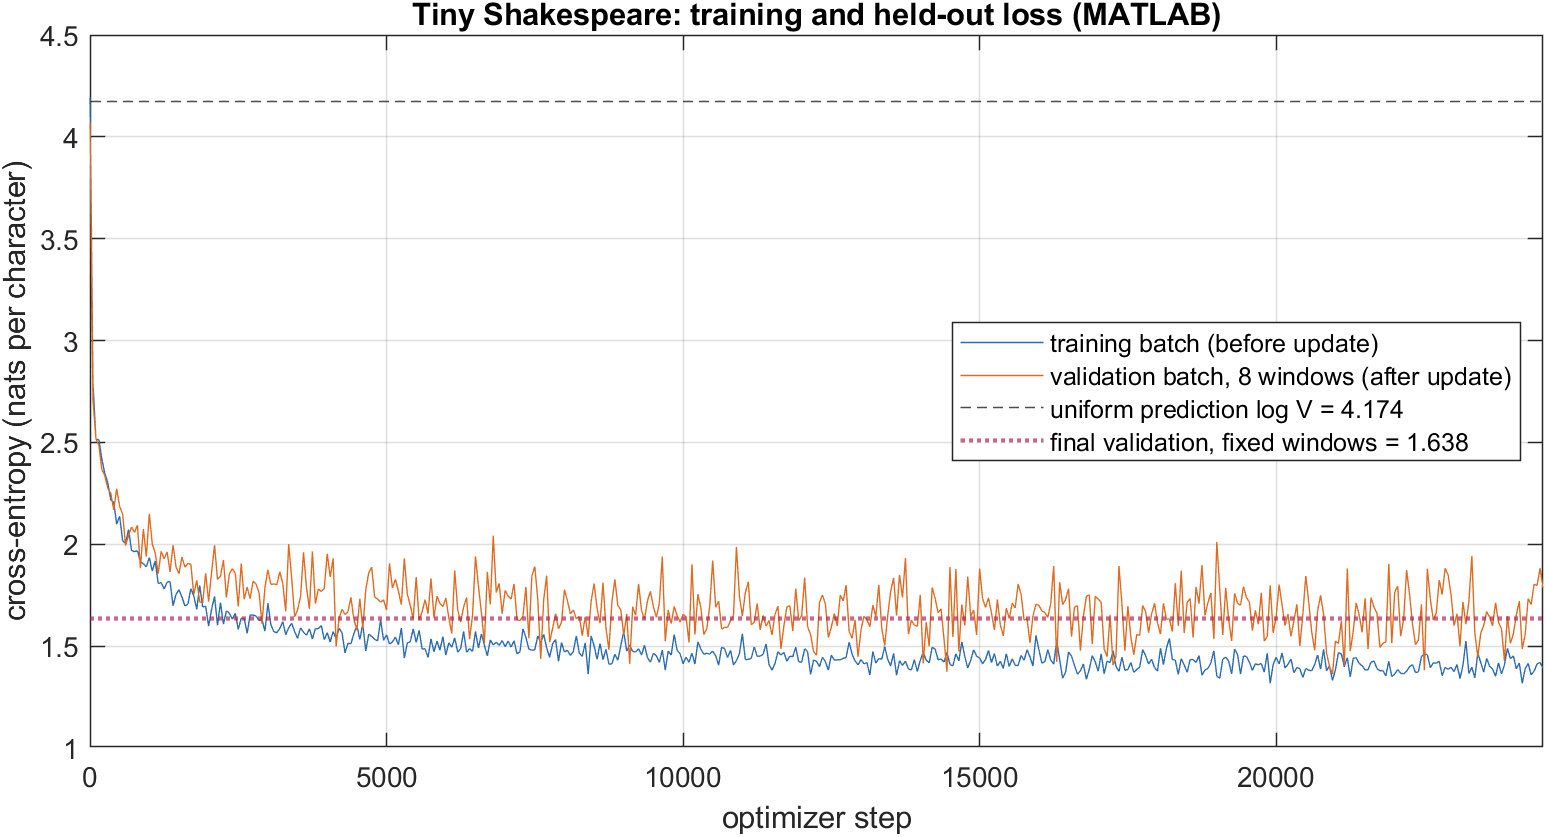
\includegraphics[width=0.8\linewidth]{loss_curves_matlab.png}
\caption{The MATLAB run: training-batch loss (before each update) and validation-batch loss (after it) at the
\NumEvals{} evaluation steps; dashed: the uniform level $\log V$; dotted: the final fixed-window validation loss.}
\label{fig:lossml}
\end{figure}
\fi

\textbf{Gradient norms.} The four groups the assignment names, at the initialization (fixed batch) and at the first and last
evaluations of training:
\begin{center}
\small
\begin{tabular}{@{}lccc@{}}
\toprule
group & initialization & step 1 & last evaluation\\ \midrule
\tabinput{generated/tab_norms.tex}
\bottomrule
\end{tabular}
\end{center}
\begin{figure}[!htb]
\centering
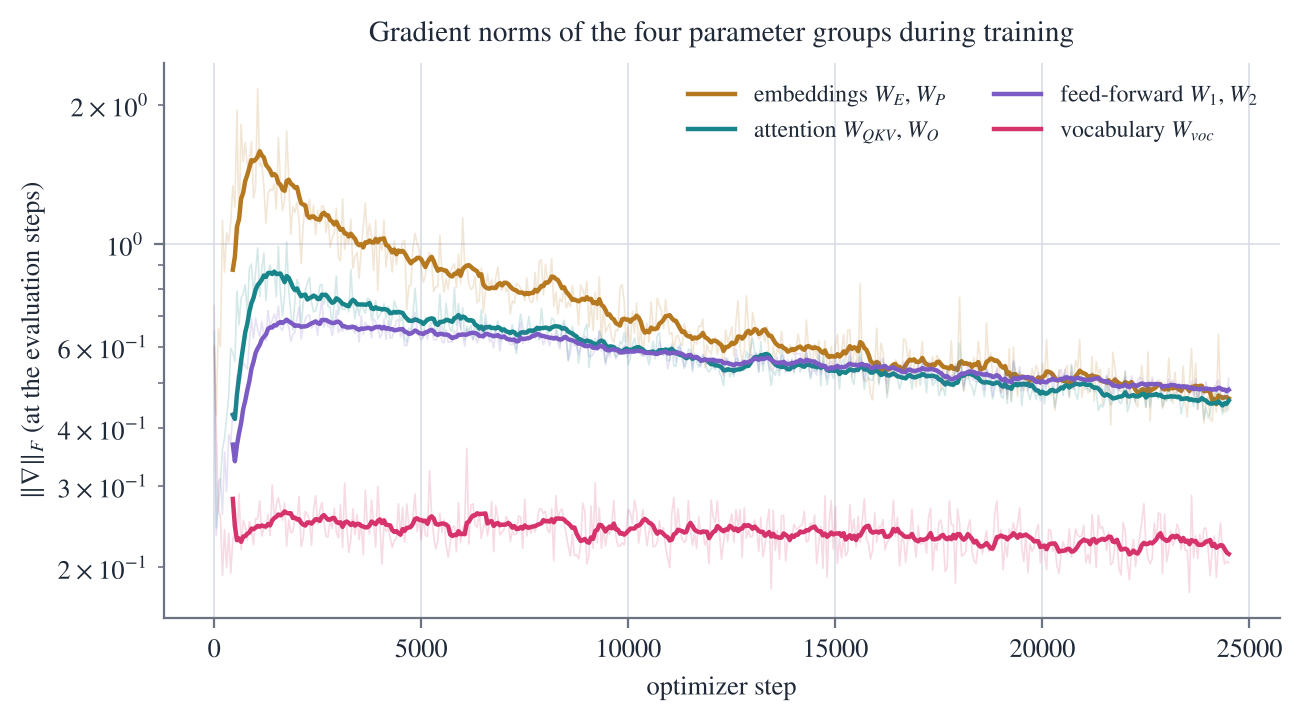
\includegraphics[width=0.72\linewidth]{grad_norms.png}
\caption{Gradient norms of the four parameter groups at the evaluation steps (faint) and their running mean.}
\label{fig:norms}
\end{figure}

\textbf{Previews during training} (80 characters from \code{ROMEO: }, every 5 epochs, categorical sampling):
\VerbatimInput{generated/previews.txt}

% =====================================================================================
\section{Question 5: autoregressive generation}\label{sec:q5}

\begin{purpose}[1. Purpose and assumptions]
A trained model gives, for any context, a distribution over the next character. Generation repeatedly samples one character,
appends it and asks again. The model only ever sees the last $T$ characters, because its position table has $T$ rows.
\end{purpose}

\stephead{2. Derivation}
For a prefix $x_{1:n}$ and continuation $x_{n+1:n+K}$,
\begin{equation}
p_\theta(x_{n+1:n+K}\mid x_{1:n})=\prod_{k=1}^{K}p_\theta\big(x_{n+k}\mid x_{\max(1,\,n+k-T):\,n+k-1}\big).
\end{equation}
At each step the retained context $x_{m:n}$, $m=\max(1,n-T+1)$, is embedded with positions $1,\dots,n-m+1$ (re-indexed from
the start of the window, because $W_P$ only has rows $1..T$ and the model was trained on windows starting at position 1).
After the blocks and $\LN_f$, only the last row matters:
\begin{equation}
z_{\rm last}=h_{\rm last}\Wvoc\in\R^{1\times V},\qquad p_j=\frac{\exp(z_j/\tau-\max_kz_k/\tau)}{\sum_q\exp(z_q/\tau-\max_kz_k/\tau)} .
\end{equation}
Row $t<n$ predicts a character that is already known; causality guarantees those rows ignore the newest token (\code{Q5.4}).
\textbf{Sampling} draws $u\sim\mathcal U(0,1)$ and returns the first index $j$ with $\sum_{q\le j}p_q>u$, so index $j$ is chosen
with probability exactly $p_j$. \textbf{Greedy decoding} returns $\arg\max_jp_j$ instead: deterministic, and prone to loops.
The required sample uses categorical sampling at $\tau=1$.

\textbf{Probability calculation} for $z=(2,1,0)$:
\begin{center}
\small
\begin{tabular}{@{}lcc@{}}
\toprule
temperature & $(p_1,p_2,p_3)$ & entropy (nats)\\ \midrule
$\tau=1$ (baseline) & \ProbOne & \EntOne\\
$\tau=0.5$ & \ProbHalf & \EntHalf\\
$\tau=2$ & \ProbTwo & \EntTwo\\
\bottomrule
\end{tabular}
\end{center}
At $\tau=1$, $p=(e^2,e,1)/(e^2+e+1)$, summing to one (\code{Q5.1}). Dividing logits by $\tau<1$ stretches their differences,
so the largest logit dominates and the entropy falls; $\tau>1$ compresses them towards uniform. In 100\,000 draws the sampler's
frequencies were \SamplerFreq{} (\code{Q5.2}).

\textbf{Context window.} For a prompt of length $T+5=69$, the next prediction keeps characters $6,7,\dots,69$ (one-based) and
places them at positions $1,\dots,64$ of $W_P$; the program's crop equals an explicit forward pass on those $T$ characters
exactly (\code{Q5.3}).

\stephead{3. Code}
\lstinputlisting[style=py,caption={Python: cropping, the categorical draw and the generation loop (\code{gpt_a2/sample.py}).}]{generated/snippets/py_sample.py}
\lstinputlisting[style=ml,caption={MATLAB: \code{generate_text.m}.}]{generated/snippets/generate_text.m}

\stephead{4. Operation-by-operation explanation}
\begin{ops}
\code{np.asarray(context)[-T:]} & \code{ids(max(1, end - T + 1):end)} & the newest $\le T$ indices; positions restart at 1\\
\code{gpt_forward(window[None, :], P, L)} & \code{gpt_forward(ctx, P, eps_ln)} & a batch of one; $Z$ has one row per position\\
\code{Z.data[-1] / temperature} & \code{Z(end, :) / temperature} & only the last row predicts the next character\\
\code{np.searchsorted(np.cumsum(p), u)} & \code{find(cumsum(p) >= rand(stream), 1)} & inverse-CDF categorical draw\\
\code{ids.append(...)}, \code{decode(...)} & \code{ids(end + 1) = nxt}; \code{decode_idx} & append, repeat, map back to characters\\
\end{ops}

\stephead{5. The generated text}
200 characters from the prompt \code{ROMEO: } with the trained model, categorical sampling, $\tau=1$, seed 454:
\VerbatimInput{generated/sample.txt}
Every generated character belongs to the corpus vocabulary (\code{Q5.5}); the output has the requested length (\code{Q5.6}).
Greedy decoding from the same prompt, for contrast:
\VerbatimInput{generated/greedy.txt}
Optional temperatures (120 characters each):
\VerbatimInput{generated/tau.txt}
\ifnum\MlRun=1
The MATLAB model (its own training run, Case~B4), the same prompt and decoding rule, MATLAB's generator with seed 454:
\VerbatimInput{generated/sample_ml.txt}
\fi

\textbf{Interpretation.} The Python sample has the local form of the corpus: capitalized speaker tags followed by a colon
and a line break (real speakers, though from different plays), short verse lines, mostly real English words with a few
invented ones, and plausible punctuation.\ifnum\MlRun=1{} The MATLAB sample has the same local form; its 200 characters
stay inside one speech, so no speaker tag appears.\fi{} \ifnum\MlRun=1 Neither has\else It lacks\fi{} long-range
coherence: no sentence carries a meaning and the speakers do not answer each other. The model conditions on at most 64 characters, has one head, two blocks and $112\,000$ parameters, so it learns which
characters follow which within words and lines, not what a sentence should mean. Greedy decoding shows the other failure
mode of a peaked distribution: it falls into a loop of high-probability phrases (``the stand of the stand of \dots'').
At $\tau=0.5$ the text is built from common words in well-formed lines; at $\tau=2$ it fills with invented spellings and
broken speaker tags.

\begin{figure}[!htb]
\centering
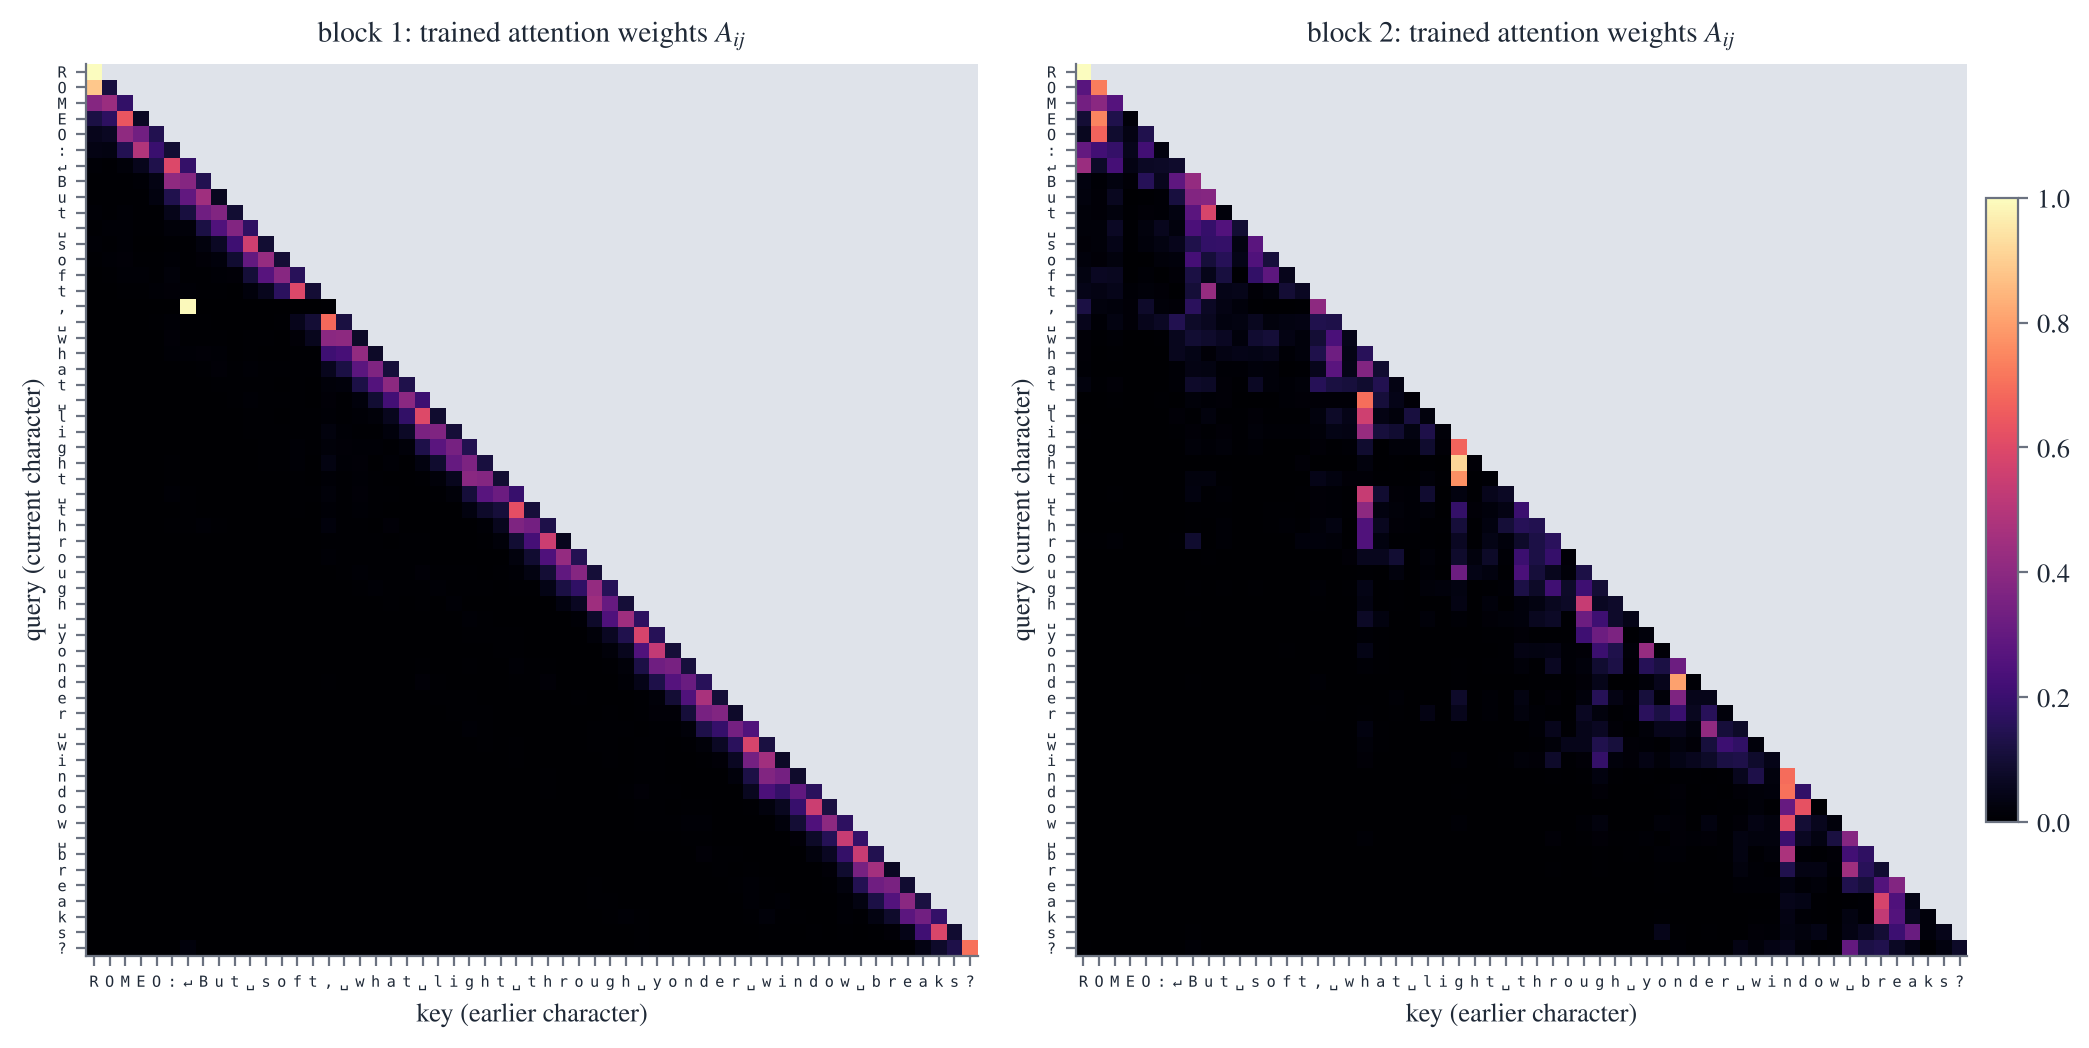
\includegraphics[width=0.98\linewidth]{attention_trained.png}
\caption{Trained attention weights of both blocks on a 56-character context (rows: the current character; columns: earlier
characters; grey: exactly zero by the causal mask).}
\label{fig:att}
\end{figure}

% =====================================================================================
\section{Question 6: integration, verification and submission}\label{sec:q6}

\subsection{The numbered checks of the assignment}
\begin{center}
\small
\begin{tabular}{@{}cp{7.4cm}p{4.2cm}c@{}}
\toprule
\# & requirement & evidence (check ids, Table~\ref{tab:checks}) & Python\\ \midrule
\tabinput{generated/tab_numbered.tex}
\bottomrule
\end{tabular}
\end{center}
The parameter table (check 1):
\begin{center}
\small
\begin{longtable}{@{}llcr@{}}
\toprule
tensor & name & shape & entries\\ \midrule\endhead
\tabinput{generated/tab_params.tex}
\midrule \textbf{total} & & & \textbf{\Ptotal}\\
\bottomrule
\end{longtable}
\end{center}
At initialization the logits of a real batch are $2048\times\Vsize$, the loss is \LzeroInit{} and $\log V=\logV$ (\code{Q6.7}):
small random weights give nearly uniform predictions. The embedding output and the block input are $32\times64\times64$
(\code{Q6.2}); the first residual sum is exactly $H^{(0)}+F$ (\code{Q6.3}); in both blocks every masked weight is exactly $0$
and every attention row sums to one within \chkpy{Q6.5} (\code{Q6.4}, \code{Q6.5}).

\subsection{Minimum acceptance tests}
Each case builds a random two-block model ($d=8$, weights $\mathcal N(0,0.5^2)$, perturbed gains and biases), computes the loss
and all gradients, changes the \emph{last} input token and compares the logits of every earlier position, and compares the
batched attention with a per-sample loop:
\begin{center}
\small
\setlength{\tabcolsep}{3.5pt}
\begin{tabular}{@{}p{5.0cm}ccccc@{}}
\toprule
case & loss & finite & \shortstack{earlier\\logits change} & \shortstack{last\\logits change} & \shortstack{vectorized\\vs loop}\\ \midrule
\tabinput{generated/tab_acceptance.tex}
\bottomrule
\end{tabular}
\end{center}
All losses and gradients are finite (\code{ACC.1}); changing a future token leaves every earlier position's logits
bit-for-bit unchanged (\code{ACC.2}) while the last position does change (\code{ACC.3}); batched and per-sample attention agree
within \chkpy{ACC.4} (\code{ACC.4}).

\subsection{Case B5 and the summary of the validation suite}
On the held-out batch of Assignment~1's protocol (32 validation windows, seed 451) and the saved Assignment~1 weights, the
standalone attention of Assignment~1 (\code{causal_self_attention} in \code{gpt_a1/model.py}) and the attention inside the
Assignment~2 block (\code{attention} in \code{gpt_a2/model.py}, and the output that \code{gpt_forward} stores) differ by at most
\BfiveErr{} (\code{B5.1}).
\begin{center}
\small
\setlength{\tabcolsep}{3.5pt}
\begin{tabular}{@{}p{0.6cm}p{0.95cm}p{2.5cm}p{2.2cm}p{3.8cm}p{4.25cm}@{}}
\toprule
case & status & what & dimensions & expected property & observed\\ \midrule
\tabinput{generated/tab_cases.tex}
\bottomrule
\end{tabular}
\end{center}
No case failed.

% =====================================================================================
\section{Table of numerical verification errors}\label{sec:table}
Every recorded check, with its pass rule and the measured value. \ifnum\MlRun=1 MATLAB uses the same ids.\else The MATLAB
column fills in when \code{results/matlab/results.json} exists and this report is rebuilt.\fi
{\small
\setlength{\tabcolsep}{4pt}
\begin{longtable}{@{}lp{6.9cm}lllc@{}}
\caption{All \NChecks{} verification checks.}\label{tab:checks}\\
\toprule
id & what is checked & pass rule & Python & MATLAB & \\ \midrule\endfirsthead
\toprule
id & what is checked & pass rule & Python & MATLAB & \\ \midrule\endhead
\tabinput{generated/tab_checks.tex}
\bottomrule
\end{longtable}}

% =====================================================================================
\section{Discussion}\label{sec:discussion}
\textbf{What the implementation establishes.} The forward pass, written once and differentiated automatically (by the
Assignment~1 engine in Python, by \code{dlgradient} in MATLAB), is the computation the assignment specifies: every
intermediate shape is checked, the hand-derived gradient of every tensor agrees with automatic differentiation to rounding
error, and both agree with centred differences at the rate the theory predicts. The deterministic cases (Benchmark B,
Case B1, the $d=2$ example) have exact answers, and \ifnum\MlRun=1 both programs reproduce\else the program reproduces\fi{} them.

\textbf{What training shows.} On the synthetic sequence the model reaches near-zero loss within a few hundred steps, so
optimization works end to end. On Tiny Shakespeare the held-out cross-entropy falls from $\log V$ to \Lvalfixed{} nats per
character (\BitsPerChar{} bits), and the samples show that the model has learned the corpus's local structure. The
generalization gap of \Lgap{} nats is moderate and has two sources: the split (the held-out plays bring new speakers and
words) and late-epoch fitting of the training text, since the validation loss stops improving well before the 50-epoch
budget ends.\ifnum\MlRun=1{} The independent MATLAB run (other initial weights, other batches) reaches \MlLvalfixed{} with
a gap of \MlLgap{} nats, so these conclusions do not hinge on one particular run.\fi

\textbf{Limitations.} \ifnum\MlRun=1 One run per language: the two final losses agree within \MlValDiff{} nats, which
suggests that the spread due to initialization and batch order is small, but two runs are not a mean with a confidence
interval\else One run, one seed: the final loss is a single measurement, not a mean with a confidence interval\fi, and
the curve depends on the random windows drawn. Two small blocks and a 64-character context limit what can be learned;
there is no dropout, weight decay, learning-rate warm-up or gradient clipping. The 8-window validation batches are noisy by
design; the fixed-window estimate reduces that noise but its windows overlap one another. Pure NumPy in double precision
makes each step slower than a framework on a GPU would be, which is why the experiment stops at the prescribed budget.

\textbf{Where the remaining error lives.} Larger context, more heads and wider blocks would let the model use longer-range
structure; weight tying ($\Wvoc=W_E\T$) would save $dV$ parameters; mini-batch noise could be reduced with larger batches or
a decaying learning rate.

% =====================================================================================
\begin{thebibliography}{9}\small
\bibitem{course} MAT 451E lecture slides and the Assignment~2 specification (B.~Uzunoğlu), ITU, 2026.
\bibitem{vaswani} A.~Vaswani et al., \emph{Attention is all you need}, NeurIPS 2017.
\bibitem{he} K.~He, X.~Zhang, S.~Ren, J.~Sun, \emph{Deep residual learning for image recognition}, CVPR 2016.
\bibitem{ba} J.~L.~Ba, J.~R.~Kiros, G.~E.~Hinton, \emph{Layer normalization}, arXiv:1607.06450, 2016.
\bibitem{gelu} D.~Hendrycks, K.~Gimpel, \emph{Gaussian error linear units (GELUs)}, arXiv:1606.08415, 2016.
\bibitem{adam} D.~P.~Kingma, J.~Ba, \emph{Adam: a method for stochastic optimization}, ICLR 2015.
\bibitem{gpt2} A.~Radford et al., \emph{Language models are unsupervised multitask learners}, OpenAI, 2019.
\bibitem{karpathy} A.~Karpathy, \emph{micrograd} and \emph{nanoGPT}, \url{https://github.com/karpathy}, and the Tiny Shakespeare corpus of \emph{char-rnn}.
\bibitem{raschka} S.~Raschka, \emph{Build a Large Language Model (From Scratch)}, Manning, 2024.
\end{thebibliography}

\end{document}
